%!TeX root = report.tex
%!TEX TS-program = pdflatex

\refstepcounter{chapter}
\addcontentsline{toc}{chapter}{\thechapter\; Механика упругого деформирования зернистых композитов со случайными размерами зерен}
\begin{center}
{\normalsize\textbf{\centering\thechapter\; МЕХАНИКА УПРУГОГО ДЕФОРМИРОВАНИЯ ЗЕРНИСТЫХ КОМПОЗИТОВ СО СЛУЧАЙНЫМИ РАЗМЕРАМИ ЗЕРЕН}}\vspace{14pt} 
\end{center}


%\chapter{Механика упругого деформирования зернистых композитов со случайными размерами зерен}

\section{Упругое состояние пространства с несколькими сферическими полостями со случайными размерами}

Рассмотрим упругое пространство с $N$ сферическими полостями, центры которых $O_j$ расположены в узлах кубической решетки со стороной $2a$ (см.~рис.~\ref{f:8:5}). Радиусы полостей будем обозначать через $R_j$. Предполагается, что $\{R_j\}_{j=1}^N$~--- случайный вектор, принадлежащий пространству $\mathbb{R}^N$, с одинаково распределенными независимыми случайными компонентами с плотностью распределения $\nu(x)$. Считается, что полости свободны о нагрузки, а на бесконечности приложено однородное напряженное состояние.

\begin{figure}[h!]
\centering
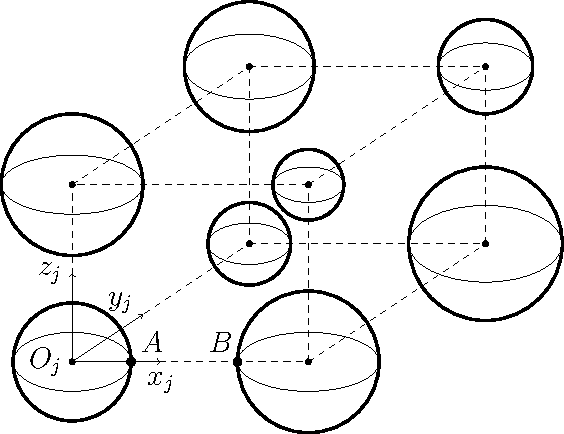
\includegraphics[width=10cm]{cartesian-spheres-stoch.pdf}
\caption{	Схематическое представление задачи}
\label{f:8:5}
\end{figure}

Введем сферические системы координат $(r_j,\theta_j,\varphi_j)$ с началами в точках $O_j$, оси которых одинаково направлены.

Соотношения между координатами можно описать формулами

\begin{equation*}
{x_i} = {r_i}\sin {\theta _i}\cos {\varphi _i},
\end{equation*}

\begin{equation}
{y_i} = {r_i}\sin {\theta _i}\sin {\varphi _i},
\label{eq:8:1}
\end{equation}

\begin{equation*}
{z_i} = {r_i}\cos {\theta _i},
\end{equation*}

\begin{equation}
\left\{ {\begin{array}{*{20}{l}}
{{x_j} = {x_\alpha } + {x_{j\alpha }},}\\
{{y_j} = {y_\alpha } + {y_{j\alpha }},}\\
{{z_j} = {z_\alpha } + {z_{j\alpha }},}
\end{array}} \right.\qquad {\kern 1pt} j \ne \alpha ,\quad j,\alpha  = \overline {1,N},
\label{eq:8:2}
\end{equation}

\noindent где $\overrightarrow {{O_j}{O_\alpha }}  = \left( {{x_{j\alpha }},{y_{j\alpha }},{z_{j\alpha }}} \right) = \left( {{r_{j\alpha }},{\theta _{j\alpha }},{\varphi _{j\alpha }}} \right)$.

Для определения НДС в рассматриваемом теле необходимо решить краевую задачу для уравнения Ламе относительно неизвестного вектора перемещения   $\mathbf{U}$ с граничными условиями

\begin{equation}
{\bf{FU}}{|_{{\Gamma _j}}} = 0
\end{equation}

\noindent и условиями на бесконечности одного из двух типов

\begin{equation}
{\bf{FU}}{|_{z =  \pm \infty }} =  \pm T{{\bf{e}}_z}\quad\text{(одноосное растяжение)},
\end{equation}

\begin{equation}
{\bf{FU}}{|_{\rho  = \infty }} = T{{\bf{e}}_\rho }\quad\text{(двуосное растяжение)},
\end{equation}

\noindent где $\mathbf{FU}$~--- отвечающий перемещению $\mathbf{U}$ вектор усилий на соответствующей граничной поверхности, ${\Gamma _j} = \left\{ {\left( {{r_j},{\theta _j},{\varphi _j}} \right):\,{r_j} = {R_j}} \right\}$.

Решение задачи будем искать в виде

\begin{equation}
{\bf{U}} = {\bf{\tilde U}} + {{\bf{U}}_0},
\end{equation}

\begin{equation}
{\bf{\tilde U}} = \sum\limits_{j = 1}^N {\sum\limits_{s = 1}^3 {\sum\limits_{n = 0}^\infty  {\sum\limits_{m =  - n - 1}^{n + 1} {a_{s,n,m}^{(j)}} } } } {\bf{\tilde U}}_{s,n,m}^{ + (4)}\left( {{r_j},{\theta _j},{\varphi _j}} \right),
\label{eq:13:7s}
\end{equation}

\begin{equation}
{{\bf{U}}_0} = \frac{T}{{2G}}\left( { - \frac{\sigma }{{1 + \sigma }}{\rho _1}{{\bf{e}}_{{\rho _1}}} + \frac{1}{{1 + \sigma }}{z_1}{{\bf{e}}_z}} \right)\quad\text{(одноосное растяжение)},
\label{eq:8:8}
\end{equation}

\begin{equation}
{{\bf{U}}_0} = \frac{T}{{2G}}\left( {\frac{{1 - \sigma }}{{1 + \sigma }}{\rho _1}{{\bf{e}}_{{\rho _1}}} - \frac{{2\sigma }}{{1 + \sigma }}{z_1}{{\bf{e}}_z}} \right)\quad\text{(двуосное растяжение)},
\label{eq:8:9}
\end{equation}

\noindent где $G$, $\sigma$~--- модуль сдвига и коэффициент Пуассона упругого пространства; $a_{s,n,m}^{(j)}$~--- неизвестные коэффициенты. Здесь и далее ${\bf{\tilde U}}_{s,n,m}^{\pm(4)}({{r_j},{\theta_j},{\varphi_j}})$~--- наборы внешних и внутренних модифицированных базисных решений уравнения Ламе в сферической системе координат. При помощи соотношений~\eqref{eq:1:89b}~--- \eqref{eq:1:99b} они связаны с со следующими частными решениями уравнения Ламе для внешности (внутренности) шара $\Omega _4^ \pm  = \left\{ {\left( {r,\theta ,\varphi } \right):{\mkern 1mu} {\kern 1pt} r \mathbin{\lower.3ex\hbox{$\buildrel>\over
{\smash{\scriptstyle<}\vphantom{_x}}$}} {r_0}} \right\}$, построенными в работе~\cite{Nikolaev1984}:

\begin{equation}
{\bf{U}}_{s,n,m}^{ \pm (4)}\left( {r,\theta ,\varphi } \right) = {{\bf{D}}_s}u_{n \mp 1,m}^{ \pm (4)}\left( {r,\theta ,\varphi } \right);\qquad {\kern 1pt} s = 1,{\mkern 1mu} {\kern 1pt} 3;
\end{equation}

\begin{equation}
{\bf{U}}_{2,n,m}^{ \pm (4)}\left( {r,\theta ,\varphi } \right) = {{\bf{D}}_2}u_{n,m}^{ \pm (4)}\left( {r,\theta ,\varphi } \right) - \frac{{r_0^2}}{{2(n \pm 1) + 1}}{{\bf{D}}_1}u_{n \pm 1,m}^{ \pm (4)}\left( {r,\theta ,\varphi } \right),
\end{equation}

\noindent где $n=0,1,\dots$, $|m|\le n+1$, $m,n\in\mathbb{Z}$.

\begin{equation}
u_{n,m}^{ \pm (4)}\left( {r,\theta ,\varphi } \right) = \left\{ \begin{array}{l}
(n - m)!/{r^{n + 1}}\\
{r^n}/(n + m)!
\end{array} \right\}P_n^m(\cos \theta ){e^{im\varphi }},\quad |m| \le n;
\end{equation}

\begin{equation*}
{{\bf{D}}_1} = \nabla  = {{\bf{e}}_x}\frac{\partial }{{\partial x}} + {{\bf{e}}_y}\frac{\partial }{{\partial y}} + {{\bf{e}}_z}\frac{\partial }{{\partial z}};\,{{\bf{D}}_2} = z\nabla  - \chi {{\bf{e}}_z};\, {{\bf{D}}_3} = i\left[ {\nabla  \times {{\bf{e}}_z}} \right],
\end{equation*}

\noindent где $\chi=3-4\sigma$; $\{\mathbf{e}_x,\mathbf{e}_y,\mathbf{e}_z\}$~--- орты декартовой системы координат.

Относительно перемещения $\mathbf{\tilde U}$ граничные условия можно записать следующим образом:

\begin{equation}
{\bf{F\tilde U}}{|_{{\Gamma _j}}} =  - {\bf{F}}{{\bf{U}}_0}{|_{{\Gamma _j}}};
\label{eq:8:5}
\end{equation}

\begin{equation}
{\bf{F\tilde U}}{|_{z =  \pm \infty }} = 0\quad\text{(одноосное растяжение)};
\label{eq:8:3}
\end{equation}

\begin{equation}
{\bf{F\tilde U}}{|_{\rho  = \infty }} = 0\quad\text{(двуосное растяжение)}.
\label{eq:8:4}
\end{equation}

Вспомогательным перемещениям $\mathbf{U}_0$ отвечают следующие напряжения на поверхностях $\Gamma_j$ ($\mathbf{n}_j=\mathbf{e}_{r_j}$~--- вектор нормали на поверхности $\Gamma_j$):

\begin{equation}
{\bf{F}}{{\bf{U}}_0} = T{P_1}(\cos {\theta _j}){{\bf{e}}_z}\quad\text{(одноосное растяжение)},
\end{equation}

\begin{equation}
{\bf{F}}{{\bf{U}}_0} =  - TP_1^{(1)}(\cos {\theta _j}){{\bf{e}}_{{\rho _j}}}\quad\text{(двуосное растяжение)}.
\end{equation}

Используя теоремы сложения, перемещение $\mathbf{\tilde U}$ можно записать полностью в системе координат с началом в точке $O_j$:

\begin{multline}
{\bf{\tilde U}} = \sum\limits_{s = 1}^3 {\sum\limits_{n = 0}^\infty  {\sum\limits_{m =  - n}^{n} {a_{s,n,m}^{(j)}} } } {\bf{\tilde U}}_{s,n,m}^{ +(4)}\left( {{r_j},{\theta _j},{\varphi _j}} \right) + \\
+ \sum\limits_{s=1}^3\sum\limits_{n = 0}^\infty\sum\limits_{m = - n}^{n}\mathbf{\tilde U}_{s,n,m}^{-(4)}(r_j,\theta_j,\varphi_j)\sum\limits_{\alpha\neq j}\sum\limits_{t=1}^3\sum\limits_{k=0}^\infty\sum\limits_{l=-k}^k\tilde T_{t,k,l,\alpha}^{s,n,m,j} a_{t,k,l}^{(\alpha)},
\label{eq:8:10}
\end{multline}
где $\tilde T_{t,k,l,\alpha}^{s,n,m,j}$ введены в формуле~\eqref{eq:1:99t}.

%\begin{equation}
%f_{n,m,j,\alpha }^{(44)k,l} = u_{n + k,m - l}^{ + (4)}\left( {{r_{j\alpha }},{\theta _{j\alpha }},{\varphi _{j\alpha }}} \right);
%\end{equation}
%
%\begin{equation}
%\tilde f_{n,m,j,\alpha }^{ - (44)k,l} = \frac{{r_{j0}^2}}{{2k + 3}}f_{n,m,j,\alpha }^{(44)k + 2,l} - {z_{j\alpha }}f_{n,m,j,\alpha }^{(44)k + 1,l} + \frac{{r_{\alpha 0}^2}}{{2n + 3}}f_{n + 1,m,j,\alpha }^{(44)k + 1,l}.
%\end{equation}

Формулы для напряжений, отвечающих базисным функциям перемещений $\mathbf{U}_{s,n,m}^{\pm(4)}(r_j,\theta_j,\varphi_j)$ на сферических поверхностях $\Gamma_j$ ($\mathbf{n}_j=\mathbf{e}_{\rho_j}$, $\mathbf{n}_j$~--- нормаль к поверхности $\Gamma_j$):

\begin{multline}
{\bf{FU}}_{1,n,m}^{ + (4)}\left( {{r_j},{\theta _j},{\varphi _j}} \right) =  - \frac{{2G}}{{{r_j}}}(n + 1)\left[ { - u_{n,m - 1}^{ + (4)}\left( {{r_j},{\theta _j},{\varphi _j}} \right){{\bf{e}}_{ - 1}} + } \right.\\
\left. { + u_{n,m + 1}^{ + (4)}\left( {{r_j},{\theta _j},{\varphi _j}} \right){{\bf{e}}_1} - u_{n,m}^{ + (4)}\left( {{r_j},{\theta _j},{\varphi _j}} \right){{\bf{e}}_0}} \right];
\label{eq:8:f1}
\end{multline}

\begin{multline}
{\bf{FU}}_{2,n,m}^{ + (4)}\left( {{r_j},{\theta _j},{\varphi _j}} \right) = \frac{{2G}}{{{r_j}}}\left\{ {(n + m)\left[ {\frac{{(n + 3)(n - m + 2)}}{{2n + 3}} - 2\sigma } \right] \times } \right.\\
\times u_{n,m - 1}^{ + (4)}\left( {{r_j},{\theta _j},{\varphi _j}} \right){{\bf{e}}_{ - 1}} - \\
- (n - m)\left[ {\frac{{(n + 3)(n + m + 2)}}{{2n + 3}} - 2\sigma } \right]u_{n,m + 1}^{ + (4)}\left( {{r_j},{\theta _j},{\varphi _j}} \right){{\bf{e}}_1} + \\
+ \left[ {\frac{{(n + 3)(n - m + 1)(n + m + 1)}}{{2n + 3}} - (n + 1)(2\sigma  - 1)} \right] \times \\
\times u_{n,m}^{ + (4)}\left( {{r_j},{\theta _j},{\varphi _j}} \right){{\bf{e}}_0} \bigg\};
\label{eq:8:f2}
\end{multline}

\begin{multline}
{\bf{FU}}_{3,n,m}^{ + (4)}\left( {{r_j},{\theta _j},{\varphi _j}} \right) =  - \frac{{2G}}{{{r_j}}}\left[ {(n - m + 2)u_{n,m - 1}^{ + (4)}\left( {{r_j},{\theta _j},{\varphi _j}} \right){{\bf{e}}_{ - 1}} + } \right.\\
\left. { + (n + m + 2)u_{n,m + 1}^{ + (4)}\left( {{r_j},{\theta _j},{\varphi _j}} \right){{\bf{e}}_1} - mu_{n,m}^{ + (4)}\left( {{r_j},{\theta _j},{\varphi _j}} \right){{\bf{e}}_0}} \right];
\label{eq:8:f3}
\end{multline}

\begin{multline}
{\bf{FU}}_{1,n,m}^{ - (4)}\left( {{r_j},{\theta _j},{\varphi _j}} \right) = \frac{{2G}}{{{r_j}}}n\bigg[ - u_{n,m - 1}^{ - (4)}\left( {{r_j},{\theta _j},{\varphi _j}} \right){{\bf{e}}_{ - 1}} + \\
+ u_{n,m + 1}^{ - (4)}\left( {{r_j},{\theta _j},{\varphi _j}} \right){{\bf{e}}_1} + u_{n,m}^{ - (4)}\left( {{r_j},{\theta _j},{\varphi _j}} \right){{\bf{e}}_0} \bigg];
\label{eq:8:f4}
\end{multline}

\begin{multline}
{\bf{FU}}_{2,n,m}^{ - (4)}\left( {{r_j},{\theta _j},{\varphi _j}} \right) = \\
= \frac{{2G}}{{{r_j}}}\left\{ { - (n - m + 1)\left[ {\frac{{(n - 2)(n + m - 1)}}{{2n - 1}} + 2\sigma } \right] \times } \right.\\
\times u_{n,m - 1}^{ - (4)}\left( {{r_j},{\theta _j},{\varphi _j}} \right){{\bf{e}}_{ - 1}} + (n + m + 1)\left[ {\frac{{(n - 2)(n - m - 1)}}{{2n - 1}} + 2\sigma } \right] \times \\
\times u_{n,m + 1}^{ + (4)}\left( {{r_j},{\theta _j},{\varphi _j}} \right){{\bf{e}}_1} + \\
\left. { + \left[ {\frac{{(n - 2)(n - m)(n + m)}}{{2n - 1}} + n(2\sigma  - 1)} \right]u_{n,m}^{ - (4)}\left( {{r_j},{\theta _j},{\varphi _j}} \right){{\bf{e}}_0}} \right\};
\label{eq:8:f5}
\end{multline}

\begin{multline}
{\bf{FU}}_{3,n,m}^{ - (4)}\left( {{r_j},{\theta _j},{\varphi _j}} \right) = \frac{{2G}}{{{r_j}}}\left[ {(n + m - 1)u_{n,m - 1}^{ - (4)}\left( {{r_j},{\theta _j},{\varphi _j}} \right){{\bf{e}}_{ - 1}} + } \right.\\
\left. { + (n - m - 1)u_{n,m + 1}^{ - (4)}\left( {{r_j},{\theta _j},{\varphi _j}} \right){{\bf{e}}_1} - mu_{n,m}^{ - (4)}\left( {{r_j},{\theta _j},{\varphi _j}} \right){{\bf{e}}_0}} \right].
\label{eq:8:f6}
\end{multline}

После перехода в формулах~\eqref{eq:8:3}, \eqref{eq:8:4} к напряжениям и удовлетворения граничным условиям относительно неизвестных $a_{s,n,m}^{(j)}$ получаем бесконечную систему линейных алгебраических уравнений:

\begin{equation}
\sum _{s=1}^3 \bigg\{a_{s,n,m}^{(j)}{\tilde F}_{s,n,m}^{+(p)}+F_{s,n,m}^{-(p)}\sum _{\alpha\neq j} \sum _{t=1}^3 \sum _{k=0}^{\infty}\sum_{l=-k}^k a_{t,k,l}^{(\alpha)} T_{t,k,l,\alpha}^{s,n,m,j}\bigg\}+F_{n,m}^{0(p)}=0;
\label{eq:13:1}
\end{equation}
$$
n,m \in\mathbb{Z}:\quad n \ge 1,{\mkern 1mu} \quad {\kern 1pt} |m| \le n - 1,\quad {\mkern 1mu} p =  1,{\mkern 1mu} {\kern 1pt} 2,{\mkern 1mu} {\kern 1pt} 3;\;\;\;{\mkern 1mu} {\kern 1pt} j = \overline {1,N},
$$

\begin{equation}
\sum _{s=1}^2 a_{s,n,n}^{(j)}{\tilde F}_{s,n,n}^{+(1)}+\sum_{s=1}^3 F_{s,n,n}^{-(1)}\sum _{\alpha\neq j} \sum _{t=1}^3 \sum _{k=0}^{\infty}\sum_{l=-k}^k a_{t,k,l}^{(\alpha)} T_{t,k,l,\alpha}^{s,n,n,j}+F_{n,n}^{0(1)}=0;
\label{eq:13:2}
\end{equation}

\begin{equation}
\sum _{s=1}^2 a_{s,n,n}^{(j)}{\tilde F}_{s,n,n}^{+(3)}+\sum_{s=1}^3 F_{s,n,n}^{-(3)}\sum _{\alpha\neq j} \sum _{t=1}^3 \sum _{k=0}^{\infty}\sum_{l=-k}^k a_{t,k,l}^{(\alpha)} T_{t,k,l,\alpha}^{s,n,n,j}+F_{n,n}^{0(3)}=0;
\label{eq:13:3}
\end{equation}

\begin{equation}
a_{3,n,n}^{(j)}{\tilde F}_{3,n,n}^{+(1)}+\sum_{s=1}^3 F_{s,n,n+1}^{-(1)}\sum _{\alpha\neq j} \sum _{t=1}^3 \sum _{k=0}^{\infty}\sum_{l=-k}^k a_{t,k,l}^{(\alpha)} T_{t,k,l,\alpha}^{s,n,n+1,j}+F_{n,n+1}^{0(1)}=0;
\label{eq:13:4}
\end{equation}

\begin{equation}
\sum _{s=1}^2 a_{s,n,-n}^{(j)}{\tilde F}_{s,n,-n}^{+(2)}+\sum_{s=1}^3 F_{s,n,-n}^{-(2)}\sum _{\alpha\neq j} \sum _{t=1}^3 \sum _{k=0}^{\infty}\sum_{l=-k}^k a_{t,k,l}^{(\alpha)} T_{t,k,l,\alpha}^{s,n,-n,j}+F_{n,-n}^{0(2)}=0;
\label{eq:13:5}
\end{equation}

\begin{equation}
\sum _{s=1}^2 a_{s,n,-n}^{(j)}{\tilde F}_{s,n,-n}^{+(3)}+\sum_{s=1}^3 F_{s,n,-n}^{-(3)}\sum _{\alpha\neq j} \sum _{t=1}^3 \sum _{k=0}^{\infty}\sum_{l=-k}^k a_{t,k,l}^{(\alpha)} T_{t,k,l,\alpha}^{s,n,-n,j}+F_{n,-n}^{0(3)}=0;
\label{eq:13:6}
\end{equation}

\begin{equation}
a_{3,n,-n}^{(j)}{\tilde F}_{3,n,-n}^{+(2)}+\sum_{s=1}^3 F_{s,n,-n-1}^{-(2)}\sum _{\alpha\neq j} \sum _{t=1}^3 \sum _{k=0}^{\infty}\sum_{l=-k}^k a_{t,k,l}^{(\alpha)} T_{t,k,l,\alpha}^{s,n,-n-1,j}+F_{n,-n-1}^{0(2)}=0;
\label{eq:13:7}
\end{equation}
$$
n\ge 1;\quad j=\overline{1,N};
$$

\begin{equation}
a_{1,0,0}^{(j)}{\tilde F}_{1,0,0}^{+(1)}+\sum_{s=1}^3 F_{s,0,1}^{-(1)}\sum _{\alpha\neq j} \sum _{t=1}^3 \sum _{k=0}^{\infty}\sum_{l=-k}^k a_{t,k,l}^{(\alpha)} T_{t,k,l,\alpha}^{s,0,1,j}+F_{0,1}^{0(1)}=0;
\label{eq:13:8}
\end{equation}

\begin{equation}
a_{2,0,0}^{(j)}{\tilde F}_{2,0,0}^{+(3)}+\sum_{s=1}^3 F_{s,0,0}^{-(3)}\sum _{\alpha\neq j} \sum _{t=1}^3 \sum _{k=0}^{\infty}\sum_{l=-k}^k a_{t,k,l}^{(\alpha)} T_{t,k,l,\alpha}^{s,0,0,j}+F_{0,0}^{0(3)}=0;
\label{eq:13:9}
\end{equation}

\begin{equation}
a_{3,0,0}^{(j)}{\tilde F}_{3,0,0}^{+(2)}+\sum_{s=1}^3 F_{s,0,-1}^{-(2)}\sum _{\alpha\neq j} \sum _{t=1}^3 \sum _{k=0}^{\infty}\sum_{l=-k}^k a_{t,k,l}^{(\alpha)} T_{t,k,l,\alpha}^{s,0,-1,j}+F_{0,-1}^{0(2)}=0;
\label{eq:13:10}
\end{equation}

%\begin{multline}
%\sum\limits_{s = 1}^3 {a_{s,n,m}^{(j)}} F_{s,n,m}^{ + (k)}({R_j}) + F_{1,n,m}^{ - (k)}({R_j})\sum\limits_{\alpha  \ne j} {\sum\limits_{k = 0}^\infty  {\sum\limits_{l =  - k - 1}^{k + 1} {{{( - 1)}^{k + m + 1}}} } \left[ {a_{1,k,l}^{(\alpha )}f_{k,l,j,\alpha }^{(44)n,m} - } \right.} \\
%\left. { - a_{2,k,l}^{(\alpha )}\tilde f_{k,l,j,\alpha }^{ - (44)n,m}} \right] + F_{2,n,m}^{ - (k)}({R_j})\sum\limits_{\alpha  \ne j} {\sum\limits_{k = 0}^\infty  {\sum\limits_{l =  - k - 1}^{k + 1} {{{( - 1)}^{k + m}}} } a_{2,k,l}^{(\alpha )}f_{k,l,j,\alpha }^{(44)n,m} + } \\
%+ F_{3,n,m}^{ - (k)}({R_j})\sum\limits_{\alpha  \ne j} \sum\limits_{k = 0}^\infty  {\sum\limits_{l =  - k - 1}^{k + 1} {{{( - 1)}^{k + m + 1}}} } a_{3,k,l}^{(\alpha )}f_{k,l,j,\alpha }^{(44)n,m} = F_{n,m}^{(k)};
%\label{eq:8:sys}
%\end{multline}
\noindent где $\tilde F_{s,n,m}^{+(p)}$~--- радиальные части компонент вектора напряжений $\mathbf{F\tilde U}_{s,n,m}^{+(4)}$ на поверхности $r_j=R_j$, отвечающего перемещению $\mathbf{\tilde U}_{s,n,m}^{+(4)}$ (выражается через $F_{s,n,m}^{+(p)}$ согласно формулам~\eqref{eq:1:89b}~--- \eqref{eq:1:99b}); 

\begin{equation}
F_{1,n,m}^{ + (2)}(R_j) = \frac{{2G}}{{{R_j^{n + 2}}}}(n + 1)(n - m + 1)!;
\label{eq:8:12}
\end{equation}
\begin{equation}
F_{1,n,m}^{ + (2)}(R_j) =  - \frac{{2G}}{{{R_j^{n + 2}}}}(n + 1)(n - m - 1)!;
\label{eq:8:12a}
\end{equation}

\begin{equation}
F_{1,n,m}^{ + (3)}(R_j) = \frac{{2G}}{{{R_j^{n + 2}}}}(n + 1)(n - m)!;
\label{eq:8:13a}
\end{equation}
\begin{equation}
F_{1,n,m}^{ + (1)}(R_j) = \frac{{2G}}{{{R_j^{n + 2}}}}(n + 1)\left[ {\frac{{(n + 3)(n - m + 2)}}{{2n + 3}} - 2\sigma } \right](n - m + 1)!;
\label{eq:8:13b}
\end{equation}
\begin{equation}
F_{2,n,m}^{ + (2)}(R_j) = - \frac{{2G}}{{{R_j^{n + 2}}}}(n - m)\left[ {\frac{{(n + 3)(n + m + 2)}}{{2n + 3}} - 2\sigma } \right](n - m - 1)!;
\label{eq:8:13c}
\end{equation}

\begin{multline}
F_{2,n,m}^{ + (3)} = \frac{{2G}}{{{R_j^{n + 2}}}}\left[ {\frac{{(n + 3)(n - m + 1)(n + m + 1)}}{{2n + 3}} - } \right.\\
\left. { - (n + 1)(2\sigma  - 1)} \right](n - m)!;
\label{eq:8:14a}
\end{multline}
\begin{equation}
F_{3,n,m}^{ + (1)}(R_j) =  - \frac{G}{{{R_j^{n + 2}}}}(n - m + 2)(n - m + 1)!;
\label{eq:8:14b}
\end{equation}
\begin{equation}
F_{3,n,m}^{ + (2)}(R_j) =  - \frac{{2G}}{{{R_j^{n + 2}}}}(n + m + 2)(n - m - 1)!;
\label{eq:8:15a}
\end{equation}
\begin{equation}
F_{3,n,m}^{ + (3)}(R_j) = \frac{G}{R_j^{n+2}}m(n - m)!;
\label{eq:8:15b}
\end{equation}
\begin{equation}
F_{1,n,m}^{ - (1)}(R_j) =  - 2G{R_j^{n - 1}}\frac{n}{{(n + m - 1)!}};
\label{eq:8:16a}
\end{equation}
\begin{equation}
F_{1,n,m}^{ - (2)}(R_j) = 2G{R_j^{n - 1}}\frac{n}{{(n + m + 1)!}};
\label{eq:8:16b}
\end{equation}
\begin{equation}
F_{1,n,m}^{ - (3)}(R_j) = 2G{R_j^{n - 1}}\frac{n}{{(n + m)!}};
\label{eq:8:17a}
\end{equation}
\begin{multline}
F_{2,n,m}^{ - (1)}(R_j) =  - 2G{R_j^{n - 1}}(n - m + 1) \times \\
\times \left[ {\frac{{(n - 2)(n + m - 1)}}{{2n - 1}} + 2\sigma } \right]\frac{1}{{(n + m - 1)!}};
\label{eq:8:17b}
\end{multline}
\begin{multline}
F_{2,n,m}^{ - (2)}(R_j) = 2G{R_j^{n - 1}}(n + m + 1)\times \\
\times\left[ {\frac{{(n - 2)(n - m - 1)}}{{2n - 1}} + 2\sigma } \right]\frac{1}{{(n + m + 1)!}};
\label{eq:8:17c}
\end{multline}

\begin{multline}
F_{2,n,m}^{ - (3)}(R_j) = 2G{R_j^{n - 1}}\times \\
\times\left[ {\frac{{(n - 2)(n - m)(n + m)}}{{2n - 1}} + n(2\sigma  - 1)} \right]\frac{1}{{(n + m)!}};
\label{eq:8:18}
\end{multline}

\begin{equation}
F_{n,m}^{0(k)} =  - T{\delta _{n1}}{\delta _{m0}}{\delta _{k3}}\quad\text{(одноосное растяжение)};
\label{eq:8:19}
\end{equation}

\begin{equation}
F_{n,m}^{0(k)} =  - T{\delta _{n1}}{\delta _{m0\,}}(2{\delta _{k1}} - {\delta _{k2}})\quad\text{(двуосное растяжение)}.
\label{eq:8:20}
\end{equation}

Введем следующие нормировки
$$
\frac{a_{s,n,m}^{(j)}}{R_j^{n+1}}=\tilde a_{s,n,m}^{(j)};\quad\tilde F_{s,n,m}^{+(p)}(R_j)R_j^{n+2}=\tilde F_{s,n,m}^{+(p)};\quad\frac{F_{s,n,m}^{-(p)}(R_j)}{R_j^{n-1}}=F_{s,n,m}^{-(p)}.
$$
Введем обозначения
$$
\tilde F(n,m)=\bigg(\tilde F_{s,n,m}^{+(p)}\bigg)_{p,s=1}^3;\quad
F(n,m)=\bigg(F_{s,n,m}^{-(p)}\bigg)_{p,s=1}^3;\quad n\ge 1, |m|\le n-1;
$$

\begin{equation*}
\tilde F(n,n)=
\begin{pmatrix}
\tilde F_{1,n,n}^{+(1)} & \tilde F_{2,n,n}^{+(1)} & 0 \\
\tilde F_{1,n,n}^{+(3)} & \tilde F_{2,n,n}^{+(3)} & 0 \\
0 & 0 & \tilde F_{3,n,n}^{+(1)}
\end{pmatrix};\quad
\tilde F(n,-n)=
\begin{pmatrix}
\tilde F_{1,n,-n}^{+(2)} & \tilde F_{2,n,-n}^{+(2)} & 0 \\
\tilde F_{1,n,-n}^{+(3)} & \tilde F_{2,n,-n}^{+(3)} & 0 \\
0 & 0 & \tilde F_{3,n,-n}^{+(2)}
\end{pmatrix};
\end{equation*}

\begin{equation*}
\tilde F(0,0)=
\begin{pmatrix}
\tilde F_{1,0,0}^{+(1)} & 0 & 0 \\
0 & \tilde F_{2,0,0}^{+(3)} & 0 \\
0 & 0 & \tilde F_{3,0,0}^{+(2)}
\end{pmatrix};\;
F^0(n,m)=\bigg(F_{n,m}^{0(p)}\bigg)_{p=1}^3;\; n\ge 1, |m|\le n-1;
\end{equation*}

\begin{equation*}
F^0(n,n)=
\begin{pmatrix}
F_{n,n}^{0(1)} \\
F_{n,n}^{0(3)} \\
F_{n,n+1}^{0(1)}
\end{pmatrix};\quad
F^0(n,-n)=
\begin{pmatrix}
F_{n,-n}^{0(2)} \\
F_{n,-n}^{0(3)} \\
F_{n,-n-1}^{0(2)}
\end{pmatrix};\quad
F^0(0,0)=
\begin{pmatrix}
F_{0,1}^{0(1)} \\
F_{0,0}^{0(3)} \\
F_{0,-1}^{0(2)}
\end{pmatrix};
\end{equation*}

\begin{equation*}
FT_{k,l,\alpha}^{n,m,j}=\bigg(FT_{t,k,l,\alpha}^{p,n,m,j}\bigg)_{p,t=1}^3;\quad
\hat T_{k,l,\alpha}^{n,m,j}=\bigg(\hat T_{t,k,l,\alpha}^{s,n,m,j}\bigg)_{s,t=1}^3;\quad
\hat T_{t,k,l,\alpha}^{s,n,m,j}=T_{t,k,l,\alpha}^{s,n,m,j} a^{n+k+1};
\end{equation*}
$$
FT_{k,l,\alpha}^{n,m,j}=F(n,m)\hat T_{k,l,\alpha}^{n,m,j};\quad n\ge 1; |m|\le n-1;
$$
$$
FT_{t,k,l,\alpha}^{p,n,n,j}=\delta_{p1}\sum_{s=1}^3 F_{s,n,n}^{-(1)}\hat T_{t,k,l,\alpha}^{s,n,n,j}+\delta_{p2}\sum_{s=1}^3 F_{s,n,n}^{-(3)}\hat T_{t,k,l,\alpha}^{s,n,n,j}+\delta_{p3}\sum_{s=1}^3 F_{s,n,n+1}^{-(1)}\hat T_{t,k,l,\alpha}^{s,n,n+1,j};
$$
\begin{multline*}
FT_{t,k,l,\alpha}^{p,n,-n,j}= \\
=\delta_{p1}\sum_{s=1}^3 F_{s,n,-n}^{-(2)}\hat T_{t,k,l,\alpha}^{s,n,-n,j}+\delta_{p2}\sum_{s=1}^3 F_{s,n,-n}^{-(3)}\hat T_{t,k,l,\alpha}^{s,n,-n,j}+\delta_{p3}\sum_{s=1}^3 F_{s,n,-n-1}^{-(2)}\hat T_{t,k,l,\alpha}^{s,n,-n-1,j};
\end{multline*}
$$
FT_{t,k,l,\alpha}^{p,0,0,j}=\delta_{p1}\sum_{s=1}^3 F_{s,0,1}^{-(1)}\hat T_{t,k,l,\alpha}^{s,0,1,j}+\delta_{p2}\sum_{s=1}^3 F_{s,0,0}^{-(3)}\hat T_{t,k,l,\alpha}^{s,0,0,j}+\delta_{p3}\sum_{s=1}^3 F_{s,0,-1}^{-(2)}\hat T_{t,k,l,\alpha}^{s,0,-1,j};
$$
$$
\tilde A^{(j)}(n,m)=\bigg(\tilde a_{s,n,m}^{(j)}\bigg)_{s=1}^3;\quad \frac{R_j}{a}=\mu_j.
$$
Тогда разрешающую систему~\eqref{eq:13:1}~--- \eqref{eq:13:10} можно записать в матричной форме

\begin{multline}
\tilde F(n,m)\tilde A^{(j)}(n,m)+\sum_{\alpha\neq j}\sum_{k=0}^\infty\sum_{l=-k}^k FT_{k,l,\alpha}^{n,m,j}\tilde A^{(\alpha)}(k,l)\mu_j^n\mu_\alpha^{k+1}+ \\
+\mu_j a F^0(n,m)=0.
\label{eq:13:52}
\end{multline}
Откуда

\begin{multline}
\tilde A^{(j)}(n,m)=-\mu_j a \tilde F^{-1}(n,m)F^0(n,m)- \\
-\mu_j^n\tilde F^{-1}(n,m)\sum_{\alpha\neq j}\sum_{k=0}^\infty\sum_{l=-k}^k FT_{k,l,\alpha}^{n,m,j}\tilde A^{(\alpha)}(k,l)\mu_\alpha^{k+1}.
\label{eq:13:53}
\end{multline}

Считая, что $\mu_j$ является малым параметром, запишем итерационное решение разрешающей системы~\eqref{eq:13:53}

\begin{equation}
\tilde A_0^{(j)}(n,m)=-\mu_j a \tilde F^{-1}(n,m)F^0(n,m);
\label{eq:13:54}
\end{equation}

\begin{multline}
\tilde A_i^{(j)}(n,m)=-\mu_j a \tilde F^{-1}(n,m)F^0(n,m)- \\
-\mu_j^n\tilde F^{-1}(n,m)\sum_{\alpha\neq j}\sum_{k=0}^\infty\sum_{l=-k}^k FT_{k,l,\alpha}^{n,m,j}\tilde A_{i-1}^{(\alpha)}(k,l)\mu_\alpha^{k+1},\quad i=\overline{1,\infty};
\label{eq:13:55}
\end{multline}
Для последовательных шагов итерации имеем

\begin{equation}
\tilde A_0^{(j)}(n,m)=-\mu_j a \tilde F^{-1}(n,m)F^0(n,m);
\label{eq:13:56}
\end{equation}

\begin{multline}
\tilde A_1^{(j)}(n,m)=-\mu_j a \tilde F^{-1}(n,m)F^0(n,m)+ \\
+a\mu_j^n\tilde F^{-1}(n,m)\sum_{\alpha\neq j}\sum_{k=0}^\infty\sum_{l=-k}^k FT_{k,l,\alpha}^{n,m,j}\tilde F^{-1}(k,l)F^0(k,l)\mu_\alpha^{k+2};
\label{eq:13:57}
\end{multline}

\begin{multline}
\tilde A_2^{(j)}(n,m)=-\mu_j a \tilde F^{-1}(n,m)F^0(n,m)+ \\
+a\mu_j^n\tilde F^{-1}(n,m)\sum_{\alpha\neq j}\sum_{k=0}^\infty\sum_{l=-k}^k FT_{k,l,\alpha}^{n,m,j}\tilde F^{-1}(k,l)F^0(k,l)\mu_\alpha^{k+2}- \\
-a\mu_j^n\tilde F^{-1}(n,m)\sum_{\alpha\neq j}\sum_{k=0}^\infty\sum_{l=-k}^k FT_{k,l,\alpha}^{n,m,j}\tilde F^{-1}(k,l)\mu_\alpha^{2k+1}\times \\
\times\sum_{\beta\neq \alpha}\sum_{r=0}^\infty\sum_{i=-r}^r FT_{r,i,\beta}^{k,l,\alpha}\tilde F^{-1}(r,i)F^0(r,i)\mu_\beta^{r+2};\quad\dots;
\label{eq:13:58}
\end{multline}
Возвращаясь к исходным обозначениям, получаем

\begin{multline}
A_1^{(j)}(n,m)=-\mu_j^{n+2} a^{n+2} \tilde F^{-1}(n,m)F^0(n,m)+ \\
+a^{n+2}\mu_j^{2n+1}\tilde F^{-1}(n,m)\sum_{\alpha\neq j}\sum_{k=0}^\infty\sum_{l=-k}^k FT_{k,l,\alpha}^{n,m,j}\tilde F^{-1}(k,l)F^0(k,l)\mu_\alpha^{k+2}.
\label{eq:13:59}
\end{multline}

Сперва будем предполагать, что плотность распределения случайного размера сферической полости является гауссовской, т.~е.
$$
\nu(x)=\frac{1}{\sqrt{2\pi}\sigma}e^{-\frac{(x-R)^2}{2\sigma^2}},
$$
где $R$~--- математическое ожидание $E[R_j]$ ($R\in [0,a]$), $\sigma$~--- среднеквадратичное отклонение случайной величины $R_j$ (выбирается таким образом, чтобы $\dfrac{a-R}{3}<\sigma<\dfrac{R}{3}$). Вычислим первый момент первого приближения к решению разрешающей системы~\eqref{eq:13:53}

\begin{multline}
E\bigg[A_1^{(j)}(n,m)\bigg]=-E\Big[\mu_j^{n+2}\Big] a^{n+2} \tilde F^{-1}(n,m)F^0(n,m)+ \\
+a^{n+2}E\Big[\mu_j^{2n+1}\Big]\tilde F^{-1}(n,m)\sum_{\alpha\neq j}\sum_{k=0}^\infty\sum_{l=-k}^k FT_{k,l,\alpha}^{n,m,j}\tilde F^{-1}(k,l)F^0(k,l)E\Big[\mu_\alpha^{k+2}\Big].
\label{eq:13:60}
\end{multline}
Здесь использован тот факт, что случайные величины $\mu_j$ и $\mu_\alpha$ независимы. Аналогично вычислим второй момент случайного вектора $A_1^{(j)}(n,m)$

\begin{multline}
E\bigg[A_1^{(j)}(n,m)\Big(A_1^{(i)}(q,p)\Big)^*\bigg]= \\
=E\Big[\mu_j^{n+2}\mu_i^{q+2}\Big] a^{n+q+4} \tilde F^{-1}(n,m)F^0(n,m)\Big(F^0(q,p)\Big)^*\Big(\tilde F^{-1}(q,p)\Big)^*- \\
-a^{n+q+4}\tilde F^{-1}(n,m)F^0(n,m)\times \\
\times\sum_{\beta\neq i}\sum_{u=0}^\infty\sum_{v=-u}^u \Big(F^0(u,v)\Big)^*\Big(\tilde F^{-1}(u,v)\Big)^*\Big(FT_{u,v,\beta}^{q,p,i}\Big)^*E\Big[\mu_j^{n+2}\mu_i^{2q+1}\mu_\beta^{u+2}\Big]\Big(\tilde F^{-1}(q,p)\Big)^*- \\
-a^{n+q+4}\tilde F^{-1}(n,m)\times \\
\times\sum_{\alpha\neq j}\sum_{k=0}^\infty\sum_{l=-k}^k FT_{k,l,\alpha}^{n,m,j}\tilde F^{-1}(k,l)F^0(k,l)E\Big[\mu_j^{2n+1}\mu_i^{q+2}\mu_\alpha^{k+2}\Big]\Big(F^0(q,p)\Big)^*\Big(\tilde F^{-1}(q,p)\Big)^*+ \\
+a^{n+q+4}\tilde F^{-1}(n,m)\times \\
\times\sum_{\alpha\neq j}\sum_{\beta\neq i}\sum_{k=0}^\infty\sum_{l=-k}^k\sum_{u=0}^\infty\sum_{v=-u}^u FT_{k,l,\alpha}^{n,m,j}\tilde F^{-1}(k,l)F^0(k,l)\Big(F^0(u,v)\Big)^*\times \\
\times\Big(\tilde F^{-1}(u,v)\Big)^*\Big(FT_{u,v,\beta}^{q,p,i}\Big)^*E\Big[\mu_j^{2n+1}\mu_i^{2q+1}\mu_\alpha^{k+2}\mu_\beta^{u+2}\Big]\Big(\tilde F^{-1}(q,p)\Big)^*.
\label{eq:13:61}
\end{multline}
При определении моментов нормального распределения используем характеристическую функцию
$$
\varphi(\lambda)=e^{i\lambda R-\frac{1}{2}\lambda^2\sigma^2}=\frac{1}{\sqrt{2\pi}\sigma}\int\limits_{-\infty}^\infty e^{i\lambda x-\frac{(x-R)^2}{2\sigma^2}}dx.
$$
Если продифференцировать обе части последнего тождества $n$ раз по $\lambda$, то получим
$$
\frac{d^n}{d\lambda^n}\bigg[e^{i\lambda R-\frac{1}{2}\lambda^2\sigma^2}\bigg]=\frac{1}{\sqrt{2\pi}\sigma}\int\limits_{-\infty}^\infty (ix)^n e^{i\lambda x-\frac{(x-R)^2}{2\sigma^2}}dx,
$$
откуда $n$-й момент нормального закона равен
$$
E\Big[R_j^n\Big]=\frac{1}{\sqrt{2\pi}\sigma}\int\limits_{-\infty}^\infty x^n e^{-\frac{(x-R)^2}{2\sigma^2}}dx=(-i)^n\bigg\{\frac{d^n}{d\lambda^n}\bigg[e^{i\lambda R-\frac{1}{2}\lambda^2\sigma^2}\bigg]\bigg\}_{\lambda=0}.
$$

Рассмотрим производящую функцию для многочленов Эрмита
$$
e^{2xt-t^2}=\sum_{n=0}^\infty\frac{H_n(x)}{n!}t^n.
$$
Тогда, подставляя $\lambda=\frac{\sqrt{2}t}{\sigma}$ в функцию $e^{i\lambda R-\frac{1}{2}\lambda^2\sigma^2}$, получаем
$$
e^{i\frac{R}{\sigma}\sqrt{2}t-t^2}=\sum_{n=0}^\infty\frac{H_n\Big(i\frac{R}{\sqrt{2}\sigma}\Big)}{n!}t^n,
$$
откуда 
$$
\bigg\{\frac{d^n}{dt^n}\bigg[e^{i\frac{R}{\sigma}\sqrt{2}t-t^2}\bigg]\bigg\}_{t=0}=H_n\bigg(\frac{R}{\sqrt{2}\sigma}i\bigg).
$$
Учитывая, что $\dfrac{d}{d\lambda}=\dfrac{\sigma}{\sqrt{2}}\dfrac{d}{dt}$, приходим к соотношению
$$
\bigg\{\frac{d^n}{d\lambda^n}\bigg[e^{i\lambda R-\frac{1}{2}\lambda^2\sigma^2}\bigg]\bigg\}_{\lambda=0}=\frac{\sigma^n}{2^\frac{n}{2}}H_n\bigg(\frac{R}{\sqrt{2}\sigma}i\bigg),
$$
т.~е.
$$
E\Big[R_j^n\Big]=\frac{(-i)^n\sigma^n}{2^\frac{n}{2}}H_n\bigg(\frac{R}{\sqrt{2}\sigma}i\bigg).
$$
Заметим, что при условии $\sigma\rightarrow 0$ из асимптотической формулы
$$
H_n(iz)\sim (2iz)^n,\quad z\rightarrow\infty
$$
следует, что
$$
\lim_{\sigma\rightarrow 0} E\Big[R_j^n\Big]=R^n.
$$

Окончательно получаем 
$$
E\Big[\mu_j^n\Big]=\frac{(-i)^n\sigma^n}{a^n 2^\frac{n}{2}}H_n\bigg(\frac{R}{\sqrt{2}\sigma}i\bigg).
$$

Подставляя этот результат в формулу~\eqref{eq:13:60}, находим первый момент случайного вектора коэффициентов при базисных решениях в формуле~\eqref{eq:13:7s}

\begin{multline}
E\bigg[A_1^{(j)}(n,m)\bigg]=-\frac{(-i)^{n+2}\sigma^{n+2}}{2^\frac{n+2}{2}}H_{n+2}\bigg(\frac{R}{\sqrt{2}\sigma}i\bigg) \tilde F^{-1}(n,m)F^0(n,m)+ \\
+\frac{(-i)^{2n+1}\sigma^{2n+1}}{a^{n-1} 2^\frac{2n+1}{2}}H_{2n+1}\bigg(\frac{R}{\sqrt{2}\sigma}i\bigg)
\tilde F^{-1}(n,m)\times \\
\times\sum_{\alpha\neq j}\sum_{k=0}^\infty\sum_{l=-k}^k FT_{k,l,\alpha}^{n,m,j}\tilde F^{-1}(k,l)F^0(k,l)
\frac{(-i)^{k+2}\sigma^{k+2}}{a^{k+2} 2^\frac{k+2}{2}}H_{k+2}\bigg(\frac{R}{\sqrt{2}\sigma}i\bigg).
\label{eq:13:62}
\end{multline}
Аналогичная подстановка в формулу~\eqref{eq:13:61} приводит ко второму моменту случайного вектора коэффициентов при базисных решениях в формуле~\eqref{eq:13:7s}. Однако ввиду ее громоздкости мы ее не приводим.

%\begin{multline}
%E\bigg[A_1^{(j)}(n,m)\Big(A_1^{(j)}(n,m)\Big)^*\bigg]= \\
%=\frac{(-1)^{n+2}\sigma^{2n+4}}{2^{n+2}}H_{2n+4}\bigg(\frac{R}{\sqrt{2}\sigma}i\bigg) 
%\tilde F^{-1}(n,m)F^0(n,m)\Big(F^0(n,m)\Big)^*\Big(\tilde F^{-1}(n,m)\Big)^*- \\
%-\frac{i^{n+1}\sigma^{3n+3}}{a^{n-1} 2^\frac{3n+3}{2}}H_{3n+3}\bigg(\frac{R}{\sqrt{2}\sigma}i\bigg)
%\tilde F^{-1}(n,m)F^0(n,m)\times \\
%\times\sum_{\alpha\neq j}\sum_{k=0}^\infty\sum_{l=-k}^k \Big(F^0(k,l)\Big)^*\Big(\tilde F^{-1}(k,l)\Big)^*\Big(FT_{k,l,\alpha}^{n,m,j}\Big)^*
%\frac{(-i)^{k+2}\sigma^{k+2}}{a^{k+2} 2^\frac{k+2}{2}}H_{k+2}\bigg(\frac{R}{\sqrt{2}\sigma}i\bigg)\times \\
%\times\Big(\tilde F^{-1}(n,m)\Big)^*-
%\frac{i^{n+1}\sigma^{3n+3}}{a^{n-1} 2^\frac{3n+3}{2}}H_{3n+3}\bigg(\frac{R}{\sqrt{2}\sigma}i\bigg)
%\tilde F^{-1}(n,m)\times \\
%\times\sum_{\alpha\neq j}\sum_{k=0}^\infty\sum_{l=-k}^k FT_{k,l,\alpha}^{n,m,j}\tilde F^{-1}(k,l)F^0(k,l)
%\frac{(-i)^{k+2}\sigma^{k+2}}{a^{k+2} 2^\frac{k+2}{2}}H_{k+2}\bigg(\frac{R}{\sqrt{2}\sigma}i\bigg)\times \\
%\times\Big(F^0(n,m)\Big)^*\Big(\tilde F^{-1}(n,m)\Big)^*
%-\frac{\sigma^{4n+2}}{a^{2n} 2^{2n+1}}H_{4n+2}\bigg(\frac{R}{\sqrt{2}\sigma}i\bigg)
%\tilde F^{-1}(n,m)\times \\
%\times\sum_{\alpha\neq j}\sum_{\beta\neq j}\sum_{k=0}^\infty\sum_{l=-k}^k\sum_{r=0}^\infty\sum_{i=-r}^r FT_{k,l,\alpha}^{n,m,j}\tilde F^{-1}(k,l)F^0(k,l)\Big(F^0(r,i)\Big)^*\times \\
%\times\Big(\tilde F^{-1}(r,i)\Big)^*\Big(FT_{r,i,\beta}^{n,m,j}\Big)^*
%\frac{(-i)^{k+r+4}\sigma^{k+r+4}}{a^{k+r+4} 2^\frac{k+r+4}{2}}\bigg[\delta_{\alpha\beta}H_{k+r+4}\bigg(\frac{R}{\sqrt{2}\sigma}i\bigg)+ \\
%+(1-\delta_{\alpha\beta})H_{k+2}\bigg(\frac{R}{\sqrt{2}\sigma}i\bigg)
%H_{r+2}\bigg(\frac{R}{\sqrt{2}\sigma}i\bigg)\bigg]
%\Big(\tilde F^{-1}(n,m)\Big)^*.
%\label{eq:13:63}
%\end{multline}

Полученные результаты можно использовать для определения математического ожидания и дисперсии компонент тензора напряжений

\begin{equation}
E\left[
\begin{pmatrix}
\sigma_x \\
\sigma_y \\
\sigma_z 
\end{pmatrix}
\right]=\sum_{j=1}^N\sum_{n=0}^\infty\sum_{m=-n}^n F_j(n,m)E\Big[A^{(j)}(n,m)\Big];
\label{eq:13:63}
\end{equation}

\begin{multline}
E\left[
\begin{pmatrix}
\sigma_x \\
\sigma_y \\
\sigma_z 
\end{pmatrix}
\begin{pmatrix}
\sigma_x &
\sigma_y &
\sigma_z 
\end{pmatrix}
\right]= \\
=\sum_{j=1}^N\sum_{n=0}^\infty\sum_{m=-n}^n
\sum_{i=1}^N\sum_{q=0}^\infty\sum_{p=-q}^q F_j(n,m)E\Big[A^{(j)}(n,m)\Big(A^{(i)}(q,p)\Big)^*\Big]\Big(F_i(q,p)\Big)^*,
\label{eq:13:64}
\end{multline}
где 
$$
F_j(n,m)=
\begin{pmatrix}
F_{1x}^{(j)}(n,m) & F_{2x}^{(j)}(n,m) & F_{3x}^{(j)}(n,m) \\
F_{1y}^{(j)}(n,m) & F_{2y}^{(j)}(n,m) & F_{3y}^{(j)}(n,m) \\
F_{1z}^{(j)}(n,m) & F_{2z}^{(j)}(n,m) & F_{3z}^{(j)}(n,m)
\end{pmatrix};
$$
$F_{sx}$, $F_{sy}$, $F_{sz}$~--- $x$-я, $y$-я, $z$-я составляющие вектора напряжений на исследуемой площадке, отвечающего перемещению $\mathbf{\tilde U}_{s,n,m}^{+(4)}$.

\begin{figure}[h!]
\centering\footnotesize
\parbox[b]{7.5cm}{\centering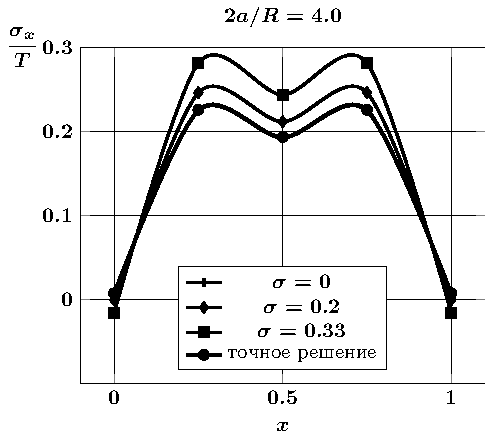
\includegraphics[width=7.5cm]{spheres-cav8-t1-sig_x-stoch.pdf}
\caption{Распределение напряжений $\sigma_x/T$ на отрезке $AB$ в зависимости от среднеквадратичного отклонения радиуса полости при одноосном растяжении 
\label{f:13:2}}}\hfil\hfil
\parbox[b]{7.5cm}{\centering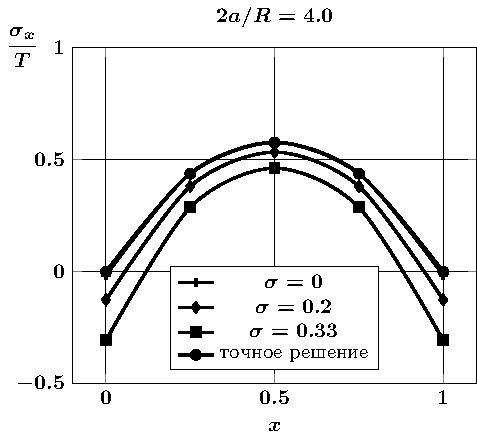
\includegraphics[width=7.5cm]{spheres-cav8-t2-sig_x-stoch.pdf}
\caption{Распределение напряжений $\sigma_x/T$ на отрезке $AB$ в зависимости от среднеквадратичного отклонения радиуса полости при двуосном растяжении
\label{f:13:3}}}
\end{figure}

На рис.~\ref{f:13:2}~--- \ref{f:13:7} представлены напряжения $\sigma_x/T$, $\sigma_y/T$ и $\sigma_z/T$ на отрезке $AB$ в зависимости от среднеквадратичного отклонения радиуса полости при одноосном и двуосном растяжении упругого пространства.
При расчетах предполагалось, что $2a/R=4.0$, число полостей $N=8$, они образуют тетрагональную упаковку, коэффициент Пуассона материала $0.38$.

Среднеквадратичное отклонение радиуса полостей $\sigma$ варьировалось в пределах от 0 до 0.33 так, что случайное изменение радиуса $R_j$ с учетом правила $3\sigma$ не выводило его за пределы отрезка $[0;a]$. Значению $\sigma=0$ отвечает случай детерминированного приближенного решения.

\begin{figure}[h!]
\centering\footnotesize
\parbox[b]{7.5cm}{\centering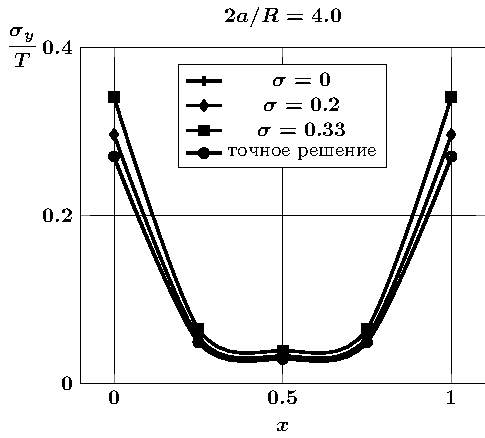
\includegraphics[width=7.3cm]{spheres-cav8-t1-sig_y-stoch.pdf}
\caption{Распределение напряжений $\sigma_y/T$ на отрезке $AB$ в зависимости от среднеквадратичного отклонения радиуса полости при одноосном растяжении 
\label{f:13:4}}}\hfil\hfil
\parbox[b]{7.5cm}{\centering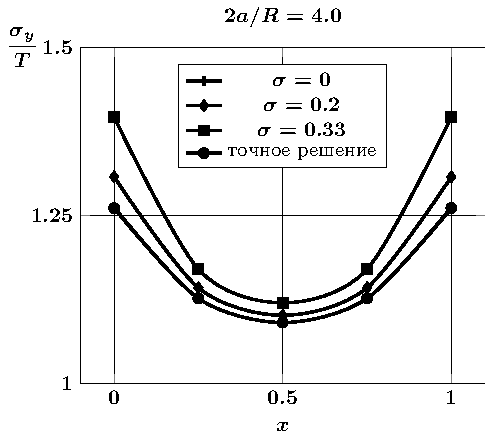
\includegraphics[width=7.3cm]{spheres-cav8-t2-sig_y-stoch.pdf}
\caption{Распределение напряжений $\sigma_y/T$ на отрезке $AB$ в зависимости от среднеквадратичного отклонения радиуса полости при двуосном растяжении
\label{f:13:5}}}
\end{figure}

\begin{figure}[h!]
\centering\footnotesize
\parbox[b]{7.5cm}{\centering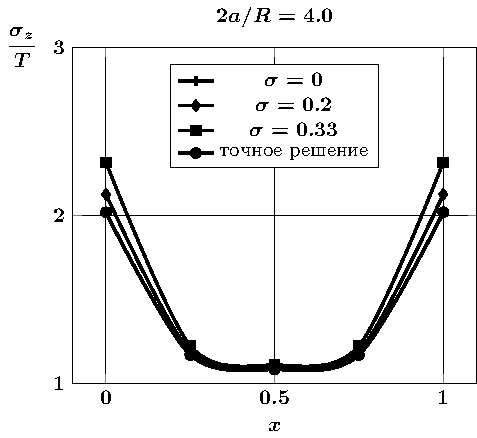
\includegraphics[width=7.3cm]{spheres-cav8-t1-sig_z-stoch.pdf}
\caption{Распределение напряжений $\sigma_z/T$ на отрезке $AB$ в зависимости от среднеквадратичного отклонения радиуса полости при одноосном растяжении 
\label{f:13:6}}}\hfil\hfil
\parbox[b]{7.5cm}{\centering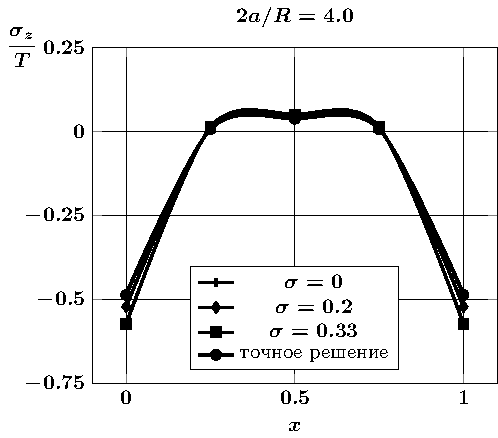
\includegraphics[width=7.3cm]{spheres-cav8-t2-sig_z-stoch.pdf}
\caption{Распределение напряжений $\sigma_z/T$ на отрезке $AB$ в зависимости от среднеквадратичного отклонения радиуса полости при двуосном растяжении
\label{f:13:7}}}
\end{figure}

На всех графиках приближенное детерминированное решение достаточно хорошо совпадает с точным. В случае $\sigma\neq 0$ наблюдается отличие в распределении напряжений стохастического и детерминированного решений. Это различие тем больше, чем больше величина $\sigma$. Наибольший разброс в значениях напряжений наблюдается при $\sigma=0.33$ и составляет 20~\% при одноосном растяжении для $\sigma_x/T$, 12~\% при двуосном растяжении для $\sigma_y/T$, 15~\% при одноосном растяжении для $\sigma_z/T$.

\section{Упругое состояние пространства с несколькими сферическими включениями со случайными размерами}

Рассмотрим упругое пространство с $N$ сферическими включениями, центры которых $O_j$ расположены в узлах кубической решетки со стороной $2a$ (см.~рис.~\ref{f:8:5}). Радиусы включений будем обозначать через $R_j$. Предполагается, что $\{R_j\}_{j=1}^N$~--- случайный вектор, принадлежащий пространству $\mathbb{R}^N$, с одинаково распределенными независимыми случайными компонентами с плотностью распределения $\nu(x)$. Считается, что включения находятся в условиях идеального контакта с матрицей, а на бесконечности приложено однородное напряженное состояние.

%\begin{figure}[h!]
%\centering
%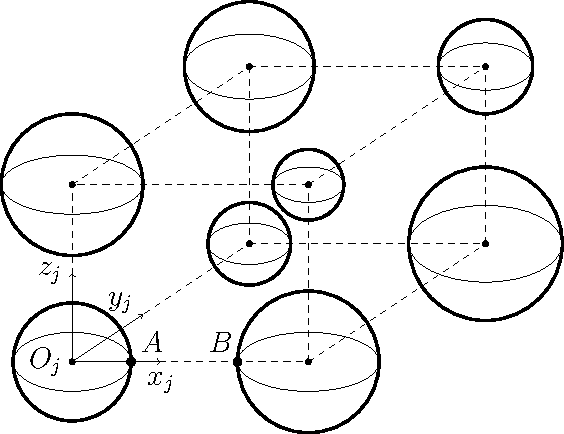
\includegraphics[width=10cm]{cartesian-spheres-stoch.pdf}
%\caption{	Схематическое представление задачи}
%\label{f:8:5}
%\end{figure}

Введем сферические системы координат $(r_j,\theta_j,\varphi_j)$ с началами в точках $O_j$, оси которых одинаково направлены.

Соотношения между координатами можно описать формулами

\begin{equation*}
{x_i} = {r_i}\sin {\theta _i}\cos {\varphi _i},
\end{equation*}

\begin{equation}
{y_i} = {r_i}\sin {\theta _i}\sin {\varphi _i},
\label{eq:8:1}
\end{equation}

\begin{equation*}
{z_i} = {r_i}\cos {\theta _i},
\end{equation*}

\begin{equation}
\left\{ {\begin{array}{*{20}{l}}
{{x_j} = {x_\alpha } + {x_{j\alpha }},}\\
{{y_j} = {y_\alpha } + {y_{j\alpha }},}\\
{{z_j} = {z_\alpha } + {z_{j\alpha }},}
\end{array}} \right.\qquad {\kern 1pt} j \ne \alpha ,\quad j,\alpha  = \overline {1,N},
\label{eq:8:2}
\end{equation}

\noindent где $\overrightarrow {{O_j}{O_\alpha }}  = \left( {{x_{j\alpha }},{y_{j\alpha }},{z_{j\alpha }}} \right) = \left( {{r_{j\alpha }},{\theta _{j\alpha }},{\varphi _{j\alpha }}} \right)$.

Предполагается, что упругие постоянные включений равны $(\sigma_j,G_j)$. Упругие постоянные матрицы будем считать равными $(\sigma,G)$.

Граничные условия~\eqref{eq:8:5} нужно заменить условиями сопряжения полей перемещений и напряжений на поверхностях $\Gamma_j$. Для того, чтобы их записать, представим вектор перемещений в упругом пространстве в виде

\begin{equation}
{\bf{U}} = \left\{ {\begin{array}{*{20}{l}}
{{\bf{\tilde U}}_j^ - ,\quad \left( {x,y,z} \right) \in {\Omega _j},}\\
{{{{\bf{\tilde U}}}^ + } + {{\bf{U}}_0},\quad \left( {x,y,z} \right) \in\mathbb{R}{^3}\backslash {\bigcup\limits_j\Omega _j},}
\end{array}} \right.
\label{eq:8:6}
\end{equation}

\noindent где ${\Omega _j} = \left\{ {\left( {{r_j},{\theta _j},{\varphi _j}} \right):\, {r_j} < {R_j}} \right\}$. Тогда условия сопряжения принимают следующий вид:

\begin{equation}
\left( {{{{\bf{\tilde U}}}^ + } + {{\bf{U}}_0}} \right){|_{{\Gamma _j}}} = {\bf{\tilde U}}_j^ - {|_{{\Gamma _j}}},
\label{eq:8:7}
\end{equation}

\begin{equation}
\left( {{\bf{F\tilde U^+}} + {\bf{F}}{{\bf{U}}_0}} \right){|_{{\Gamma _j}}} = {\bf{F}}{{\bf{\tilde U^-}}_j}{|_{{\Gamma _j}}},\qquad {\kern 1pt} j = 1,{\mkern 1mu} {\kern 1pt} 2,\dots.
\label{eq:8:11}
\end{equation}

В формулах~\eqref{eq:8:6}, \eqref{eq:8:7} вектор $\mathbf{U}_0$ определен в~\eqref{eq:8:8}, \eqref{eq:8:9}. Вектор-функции $\mathbf{\tilde U}^+$, $\mathbf{\tilde U}_j^-$ будем искать в виде

\begin{equation}
{{\bf{\tilde U}}^ + } = \mathop \sum \limits_{j = 1}^N \sum\limits_{s = 1}^3 {\sum\limits_{n = 0}^\infty  {\sum\limits_{m =  - n }^{n} {a_{s,n,m}^{(j)}} } } {\bf{\tilde U}}_{s,n,m}^{ + (4)}\left( {{r_j},{\theta _j},{\varphi _j}} \right),
\end{equation}

\begin{equation}
{\bf{\tilde U}}_j^ -  = \sum\limits_{s = 1}^3 {\sum\limits_{n = 0}^\infty  {\sum\limits_{m =  - n}^{n} {b_{s,n,m}^{(j)}} } } {\bf{\tilde U}}_{s,n,m}^{ - (4)}\left( {{r_j},{\theta _j},{\varphi _j}} \right),
\end{equation}

\noindent где $a_{s,n,m}^{(j)}$, $b_{s,n,m}^{(j)}$~--- неизвестные коэффициенты.

Для представления вектора перемещений $\mathbf{\tilde U}^+$ в системах координат с началами $O_j$ можем использовать формулы~\eqref{eq:8:10}.

После перехода в формулах~\eqref{eq:8:7}, \eqref{eq:8:11} к напряжениям и удовлетворения граничным условиям относительно неизвестных $a_{s,n,m}^{(j)}$, $b_{s,n,m}^{(j)}$ получаем бесконечную систему линейных алгебраических уравнений:

\begin{multline}
\sum_{s=1}^3 \bigg\{a_{s,n,m}^{(j)}{\tilde F}_{s,n,m}^{+(p)}+F_{s,n,m}^{-(p)}\sum _{\alpha\neq j} \sum _{t=1}^3 \sum _{k=0}^{\infty}\sum_{l=-k}^k a_{t,k,l}^{(\alpha)} T_{t,k,l,\alpha}^{s,n,m,j}\bigg\}+F_{n,m}^{0(p)}= \\
=\frac{G_j}{G}\sum_{s=1}^3 b_{s,n,m}^{(j)}{\tilde F}_{s,n,m}^{-(p)};
\label{eq:13:1a}
\end{multline}

\begin{multline}
\sum_{s=1}^2 a_{s,n,n}^{(j)}{\tilde F}_{s,n,n}^{+(1)}+\sum_{s=1}^3 F_{s,n,n}^{-(1)}\sum _{\alpha\neq j} \sum _{t=1}^3 \sum _{k=0}^{\infty}\sum_{l=-k}^k a_{t,k,l}^{(\alpha)} T_{t,k,l,\alpha}^{s,n,n,j}+F_{n,n}^{0(1)}= \\
=\frac{G_j}{G}\bigg(b_{1,n,n}^{(j)}{\tilde F}_{1,n,n}^{-(1)}+b_{3,n,n}^{(j)}{\tilde F}_{3,n,n}^{-(1)}\bigg);
\label{eq:13:2a}
\end{multline}

\begin{multline}
\sum _{s=1}^2 a_{s,n,n}^{(j)}{\tilde F}_{s,n,n}^{+(3)}+\sum_{s=1}^3 F_{s,n,n}^{-(3)}\sum _{\alpha\neq j} \sum _{t=1}^3 \sum _{k=0}^{\infty}\sum_{l=-k}^k a_{t,k,l}^{(\alpha)} T_{t,k,l,\alpha}^{s,n,n,j}+F_{n,n}^{0(3)}= \\
=\frac{G_j}{G}\bigg(b_{1,n,n}^{(j)}{\tilde F}_{1,n,n}^{-(3)}+b_{3,n,n}^{(j)}{\tilde F}_{3,n,n}^{-(3)}\bigg);
\label{eq:13:3a}
\end{multline}

\begin{multline}
a_{3,n,n}^{(j)}{\tilde F}_{3,n,n}^{+(1)}+\sum_{s=1}^3 F_{s,n,n+1}^{-(1)}\sum _{\alpha\neq j} \sum _{t=1}^3 \sum _{k=0}^{\infty}\sum_{l=-k}^k a_{t,k,l}^{(\alpha)} T_{t,k,l,\alpha}^{s,n,n+1,j}+F_{n,n+1}^{0(1)}= \\
=\frac{G_j}{G}b_{2,n,n}^{(j)}{\tilde F}_{2,n,n}^{-(1)};
\label{eq:13:4a}
\end{multline}

\begin{multline}
\sum _{s=1}^2 a_{s,n,-n}^{(j)}{\tilde F}_{s,n,-n}^{+(2)}+\sum_{s=1}^3 F_{s,n,-n}^{-(2)}\sum _{\alpha\neq j} \sum _{t=1}^3 \sum _{k=0}^{\infty}\sum_{l=-k}^k a_{t,k,l}^{(\alpha)} T_{t,k,l,\alpha}^{s,n,-n,j}+F_{n,-n}^{0(2)}= \\
=\frac{G_j}{G}\bigg(b_{1,n,-n}^{(j)}{\tilde F}_{1,n,-n}^{-(2)}+b_{3,n,-n}^{(j)}{\tilde F}_{3,n,-n}^{-(2)}\bigg);
\label{eq:13:5a}
\end{multline}

\begin{multline}
\sum _{s=1}^2 a_{s,n,-n}^{(j)}{\tilde F}_{s,n,-n}^{+(3)}+\sum_{s=1}^3 F_{s,n,-n}^{-(3)}\sum _{\alpha\neq j} \sum _{t=1}^3 \sum _{k=0}^{\infty}\sum_{l=-k}^k a_{t,k,l}^{(\alpha)} T_{t,k,l,\alpha}^{s,n,-n,j}+F_{n,-n}^{0(3)}= \\
=\frac{G_j}{G}\bigg(b_{1,n,-n}^{(j)}{\tilde F}_{1,n,-n}^{-(3)}+b_{3,n,-n}^{(j)}{\tilde F}_{3,n,-n}^{-(3)}\bigg);
\label{eq:13:6a}
\end{multline}

\begin{multline}
a_{3,n,-n}^{(j)}{\tilde F}_{3,n,-n}^{+(2)}+\sum_{s=1}^3 F_{s,n,-n-1}^{-(2)}\sum _{\alpha\neq j} \sum _{t=1}^3 \sum _{k=0}^{\infty}\sum_{l=-k}^k a_{t,k,l}^{(\alpha)} T_{t,k,l,\alpha}^{s,n,-n-1,j}+F_{n,-n-1}^{0(2)}= \\
=\frac{G_j}{G}b_{2,n,-n}^{(j)}{\tilde F}_{2,n,-n}^{-(2)};
\label{eq:13:7a}
\end{multline}

\begin{multline}
a_{1,0,0}^{(j)}{\tilde F}_{1,0,0}^{+(1)}+\sum_{s=1}^3 F_{s,0,1}^{-(1)}\sum _{\alpha\neq j} \sum _{t=1}^3 \sum _{k=0}^{\infty}\sum_{l=-k}^k a_{t,k,l}^{(\alpha)} T_{t,k,l,\alpha}^{s,0,1,j}+F_{0,1}^{0(1)}= \\
=\frac{G_j}{G}b_{2,0,0}^{(j)}{\tilde F}_{2,0,0}^{-(1)};
\label{eq:13:8a}
\end{multline}

\begin{multline}
a_{2,0,0}^{(j)}{\tilde F}_{2,0,0}^{+(3)}+\sum_{s=1}^3 F_{s,0,0}^{-(3)}\sum _{\alpha\neq j} \sum _{t=1}^3 \sum _{k=0}^{\infty}\sum_{l=-k}^k a_{t,k,l}^{(\alpha)} T_{t,k,l,\alpha}^{s,0,0,j}+F_{0,0}^{0(3)}= \\
=\frac{G_j}{G}b_{1,0,0}^{(j)}{\tilde F}_{1,0,0}^{-(3)};
\label{eq:13:9a}
\end{multline}

\begin{multline}
a_{3,0,0}^{(j)}{\tilde F}_{3,0,0}^{+(2)}+\sum_{s=1}^3 F_{s,0,-1}^{-(2)}\sum _{\alpha\neq j} \sum _{t=1}^3 \sum _{k=0}^{\infty}\sum_{l=-k}^k a_{t,k,l}^{(\alpha)} T_{t,k,l,\alpha}^{s,0,-1,j}+F_{0,-1}^{0(2)}= \\
=\frac{G_j}{G}b_{3,0,0}^{(j)}{\tilde F}_{3,0,0}^{-(2)};
\label{eq:13:10a}
\end{multline}

\begin{multline}
\sum_{s=1}^3 \bigg\{a_{s,n,m}^{(j)}{\tilde E}_{s,n,m}^{+(p)}+E_{s,n,m}^{-(p)}\sum _{\alpha\neq j} \sum _{t=1}^3 \sum _{k=0}^{\infty}\sum_{l=-k}^k a_{t,k,l}^{(\alpha)} T_{t,k,l,\alpha}^{s,n,m,j}\bigg\}+E_{n,m}^{0(p)}= \\
=\sum_{s=1}^3 b_{s,n,m}^{(j)}{\tilde E}_{s,n,m}^{-(p)};
\label{eq:13:1b}
\end{multline}

\begin{multline}
\sum_{s=1}^2 a_{s,n,n}^{(j)}{\tilde E}_{s,n,n}^{+(1)}+\sum_{s=1}^3 E_{s,n,n}^{-(1)}\sum _{\alpha\neq j} \sum _{t=1}^3 \sum _{k=0}^{\infty}\sum_{l=-k}^k a_{t,k,l}^{(\alpha)} T_{t,k,l,\alpha}^{s,n,n,j}+E_{n,n}^{0(1)}= \\
=b_{1,n,n}^{(j)}{\tilde E}_{1,n,n}^{-(1)}+b_{3,n,n}^{(j)}{\tilde E}_{3,n,n}^{-(1)};
\label{eq:13:2b}
\end{multline}

\begin{multline}
\sum _{s=1}^2 a_{s,n,n}^{(j)}{\tilde E}_{s,n,n}^{+(3)}+\sum_{s=1}^3 E_{s,n,n}^{-(3)}\sum _{\alpha\neq j} \sum _{t=1}^3 \sum _{k=0}^{\infty}\sum_{l=-k}^k a_{t,k,l}^{(\alpha)} T_{t,k,l,\alpha}^{s,n,n,j}+E_{n,n}^{0(3)}= \\
=b_{1,n,n}^{(j)}{\tilde E}_{1,n,n}^{-(3)}+b_{3,n,n}^{(j)}{\tilde E}_{3,n,n}^{-(3)};
\label{eq:13:3b}
\end{multline}

\begin{multline}
a_{3,n,n}^{(j)}{\tilde E}_{3,n,n}^{+(1)}+\sum_{s=1}^3 E_{s,n,n+1}^{-(1)}\sum _{\alpha\neq j} \sum _{t=1}^3 \sum _{k=0}^{\infty}\sum_{l=-k}^k a_{t,k,l}^{(\alpha)} T_{t,k,l,\alpha}^{s,n,n+1,j}+E_{n,n+1}^{0(1)}= \\
=b_{2,n,n}^{(j)}{\tilde E}_{2,n,n}^{-(1)};
\label{eq:13:4b}
\end{multline}

\begin{multline}
\sum _{s=1}^2 a_{s,n,-n}^{(j)}{\tilde E}_{s,n,-n}^{+(2)}+\sum_{s=1}^3 E_{s,n,-n}^{-(2)}\sum _{\alpha\neq j} \sum _{t=1}^3 \sum _{k=0}^{\infty}\sum_{l=-k}^k a_{t,k,l}^{(\alpha)} T_{t,k,l,\alpha}^{s,n,-n,j}+E_{n,-n}^{0(2)}= \\
=b_{1,n,-n}^{(j)}{\tilde E}_{1,n,-n}^{-(2)}+b_{3,n,-n}^{(j)}{\tilde E}_{3,n,-n}^{-(2)};
\label{eq:13:5b}
\end{multline}

\begin{multline}
\sum _{s=1}^2 a_{s,n,-n}^{(j)}{\tilde E}_{s,n,-n}^{+(3)}+\sum_{s=1}^3 E_{s,n,-n}^{-(3)}\sum _{\alpha\neq j} \sum _{t=1}^3 \sum _{k=0}^{\infty}\sum_{l=-k}^k a_{t,k,l}^{(\alpha)} T_{t,k,l,\alpha}^{s,n,-n,j}+E_{n,-n}^{0(3)}= \\
=b_{1,n,-n}^{(j)}{\tilde E}_{1,n,-n}^{-(3)}+b_{3,n,-n}^{(j)}{\tilde E}_{3,n,-n}^{-(3)};
\label{eq:13:6b}
\end{multline}

\begin{multline}
a_{3,n,-n}^{(j)}{\tilde E}_{3,n,-n}^{+(2)}+\sum_{s=1}^3 E_{s,n,-n-1}^{-(2)}\sum _{\alpha\neq j} \sum _{t=1}^3 \sum _{k=0}^{\infty}\sum_{l=-k}^k a_{t,k,l}^{(\alpha)} T_{t,k,l,\alpha}^{s,n,-n-1,j}+E_{n,-n-1}^{0(2)}= \\
=b_{2,n,-n}^{(j)}{\tilde E}_{2,n,-n}^{-(2)};
\label{eq:13:7b}
\end{multline}

\begin{equation}
a_{1,0,0}^{(j)}{\tilde E}_{1,0,0}^{+(1)}+\sum_{s=1}^3 E_{s,0,1}^{-(1)}\sum _{\alpha\neq j} \sum _{t=1}^3 \sum _{k=0}^{\infty}\sum_{l=-k}^k a_{t,k,l}^{(\alpha)} T_{t,k,l,\alpha}^{s,0,1,j}+E_{0,1}^{0(1)}=b_{2,0,0}^{(j)}{\tilde E}_{2,0,0}^{-(1)};
\label{eq:13:8b}
\end{equation}

\begin{equation}
a_{2,0,0}^{(j)}{\tilde E}_{2,0,0}^{+(3)}+\sum_{s=1}^3 E_{s,0,0}^{-(3)}\sum _{\alpha\neq j} \sum _{t=1}^3 \sum _{k=0}^{\infty}\sum_{l=-k}^k a_{t,k,l}^{(\alpha)} T_{t,k,l,\alpha}^{s,0,0,j}+E_{0,0}^{0(3)}=b_{1,0,0}^{(j)}{\tilde E}_{1,0,0}^{-(3)};
\label{eq:13:9b}
\end{equation}

\begin{equation}
a_{3,0,0}^{(j)}{\tilde E}_{3,0,0}^{+(2)}+\sum_{s=1}^3 E_{s,0,-1}^{-(2)}\sum _{\alpha\neq j} \sum _{t=1}^3 \sum _{k=0}^{\infty}\sum_{l=-k}^k a_{t,k,l}^{(\alpha)} T_{t,k,l,\alpha}^{s,0,-1,j}+E_{0,-1}^{0(2)}=b_{3,0,0}^{(j)}{\tilde E}_{3,0,0}^{-(2)};
\label{eq:13:10b}
\end{equation}
где $\tilde F_{s,n,m}^{\pm (p)}$~--- радиальные части компонент вектора напряжений $\mathbf{F\tilde U}_{s,n,m}^{\pm (4)}$ на поверхности $r_j=R_j$, отвечающего перемещению $\mathbf{\tilde U}_{s,n,m}^{\pm (4)}$; $\tilde E_{s,n,m}^{\pm (p)}$~--- радиальные части компонент вектора перемещений $\mathbf{\tilde U}_{s,n,m}^{\pm (4)}$ на поверхности $r_j=R_j$ (выражаются через $F_{s,n,m}^{\pm (p)}$  и $E_{s,n,m}^{\pm (p)}$ согласно формулам~\eqref{eq:1:89b}~--- \eqref{eq:1:99b}). 
$$
E_{1,n,m}^{ \pm (1)}(R_j) =  - \tilde u_{n,m - 1}^{ \pm (4)}(R_j),\quad
E_{1,n,m}^{ \pm (2)}(R_j) = \tilde u_{n,m + 1}^{ \pm (4)}(R_j),\quad
E_{1,n,m}^{ \pm (3)}(R_j) =  \mp \tilde u_{n,m}^{ \pm (4)}(R_j);
$$
$$
E_{2,n,m}^{ + (1)}(R_j) =  - \frac{{(n - m + 2)(n + m)}}{{2n + 3}}\tilde u_{n,m - 1}^{ + (4)}(R_j);
$$
$$
E_{2,n,m}^{ + (2)}(R_j) = \frac{{(n - m)(n + m + 2)}}{{2n + 3}}\tilde u_{n,m + 1}^{ + (4)}(R_j);
$$
$$
E_{2,n,m}^{ + (3)}(R_j) =  - \left[ {\frac{{(n - m + 1)(n + m + 1)}}{{2n + 3}} + {\chi}} \right]\tilde u_{n,m}^{ + (4)}(R_j);
$$
$$
E_{2,n,m}^{ - (1)}(R_j) =  - \frac{{(n - m + 1)(n + m - 1)}}{{2n - 1}}\tilde u_{n,m - 1}^{ - (4)}(R_j);
$$
$$
E_{2,n,m}^{ - (2)}(R_j) = \frac{{(n - m - 1)(n + m + 1)}}{{2n - 1}}\tilde u_{n,m + 1}^{ - (4)}(R_j);
$$
$$
E_{2,n,m}^{ - (3)}(R_j) = \left[ {\frac{{(n - m)(n + m)}}{{2n - 1}} - {\chi}} \right]\tilde u_{n,m}^{ - (4)}(R_j);
$$
$$
E_{3,n,m}^{ \pm (1)}(R_j) =  - \tilde u_{n,m - 1}^{ \pm (4)}(R_j);\quad
E_{3,n,m}^{ \pm (2)}(R_j) =  - \tilde u_{n,m + 1}^{ \pm (4)}(R_j);\quad
E_{3,n,m}^{ \pm (3)}(R_j) = 0;
$$
$$
\tilde u_{n,m}^{ \pm (4)}(R) = \left\{ \begin{array}{l}
\dfrac{{(n - m)!}}{{{R^{n + 1}}}}\\
\dfrac{{{R^n}}}{{(n + m)!}}
\end{array} \right\};
$$
$$
E_{n,m}^{0(p)}=\frac{T}{2G(\sigma+1)}\delta_{n1}\delta_{m0}(-2\sigma\delta_{p1}+\sigma\delta_{p2}+\delta_{p3})\quad\text{(одноосное растяжение)};
$$
$$
E_{n,m}^{0(p)}=\frac{T}{2G(\sigma+1)}\delta_{n1}\delta_{m0}\big((2-2\sigma)\delta_{p1}+(\sigma-1)\delta_{p2}-
2\sigma\delta_{p3}\big)
\quad\text{(двуосное растяжение)}.
$$

Введем следующие нормировки
$$
\frac{a_{s,n,m}^{(j)}}{R_j^{n+1}}=\tilde a_{s,n,m}^{(j)};\quad b_{s,n,m}^{(j)}R_j^n=\tilde b_{s,n,m}^{(j)};
$$
$$
\tilde F_{s,n,m}^{+(p)}(R_j)R_j^{n+2}=\tilde F_{s,n,m}^{+(p)};\quad\frac{F_{s,n,m}^{-(p)}(R_j)}{R_j^{n-1}}=F_{s,n,m}^{-(p)};\quad\frac{\tilde F_{s,n,m}^{-(p)}(R_j)}{R_j^{n-1}}=\tilde F_{s,n,m}^{-(p)};
$$
$$
\tilde E_{s,n,m}^{+(p)}(R_j)R_j^{n+1}=\tilde E_{s,n,m}^{+(p)};\quad\frac{E_{s,n,m}^{-(p)}(R_j)}{R_j^n}=E_{s,n,m}^{-(p)};\quad\frac{\tilde E_{s,n,m}^{-(p)}(R_j)}{R_j^n}=\tilde E_{s,n,m}^{-(p)}.
$$

Введем обозначения
$$
\hat F(n,m)=\frac{G_j}{G}\bigg(\tilde F_{s,n,m}^{-(p)}\bigg)_{p,s=1}^3;\quad n\ge 1, |m|\le n-1;
$$

\begin{equation*}
\hat F(n,n)=\frac{G_j}{G}
\begin{pmatrix}
\tilde F_{1,n,n}^{-(1)} & 0 & \tilde F_{3,n,n}^{-(1)} \\
\tilde F_{1,n,n}^{-(3)} & 0 & \tilde F_{3,n,n}^{-(3)} \\
0 & \tilde F_{2,n,n}^{-(1)} & 0
\end{pmatrix};
\hat F(n,-n)=\frac{G_j}{G}
\begin{pmatrix}
\tilde F_{1,n,-n}^{-(1)} & 0 & \tilde F_{3,n,-n}^{-(1)} \\
\tilde F_{1,n,-n}^{-(3)} & 0 & \tilde F_{3,n,-n}^{-(3)} \\
0 & \tilde F_{2,n,-n}^{-(1)} & 0
\end{pmatrix};
\end{equation*}

\begin{equation*}
\hat F(0,0)=\frac{G_j}{G}
\begin{pmatrix}
0 & \tilde F_{2,0,0}^{-(1)} & 0 \\
\tilde F_{1,0,0}^{-(3)} & 0 & 0 \\
0 & 0 & \tilde F_{3,0,0}^{-(2)}
\end{pmatrix};\;
E^0(n,m)=\bigg(E_{n,m}^{0(p)}\bigg)_{p=1}^3;\; n\ge 1, |m|\le n-1;
\end{equation*}

\begin{equation*}
E^0(n,n)=
\begin{pmatrix}
E_{n,n}^{0(1)} \\
E_{n,n}^{0(3)} \\
E_{n,n+1}^{0(1)}
\end{pmatrix};\quad
E^0(n,-n)=
\begin{pmatrix}
E_{n,-n}^{0(2)} \\
E_{n,-n}^{0(3)} \\
E_{n,-n-1}^{0(2)}
\end{pmatrix};\quad
E^0(0,0)=
\begin{pmatrix}
E_{0,1}^{0(1)} \\
E_{0,0}^{0(3)} \\
E_{0,-1}^{0(2)}
\end{pmatrix};
\end{equation*}

$$
\tilde E(n,m)=\bigg(\tilde E_{s,n,m}^{+(p)}\bigg)_{p,s=1}^3;\quad
E(n,m)=\bigg(E_{s,n,m}^{-(p)}\bigg)_{p,s=1}^3;\quad n\ge 1, |m|\le n-1;
$$

\begin{equation*}
\tilde E(n,n)=
\begin{pmatrix}
\tilde E_{1,n,n}^{+(1)} & \tilde E_{2,n,n}^{+(1)} & 0 \\
\tilde E_{1,n,n}^{+(3)} & \tilde E_{2,n,n}^{+(3)} & 0 \\
0 & 0 & \tilde E_{3,n,n}^{+(1)}
\end{pmatrix};\quad
\tilde E(n,-n)=
\begin{pmatrix}
\tilde E_{1,n,-n}^{+(2)} & \tilde E_{2,n,-n}^{+(2)} & 0 \\
\tilde E_{1,n,-n}^{+(3)} & \tilde E_{2,n,-n}^{+(3)} & 0 \\
0 & 0 & \tilde E_{3,n,-n}^{+(2)}
\end{pmatrix};
\end{equation*}

\begin{equation*}
\tilde E(0,0)=
\begin{pmatrix}
\tilde E_{1,0,0}^{+(1)} & 0 & 0 \\
0 & \tilde E_{2,0,0}^{+(3)} & 0 \\
0 & 0 & \tilde E_{3,0,0}^{+(2)}
\end{pmatrix};
\end{equation*}

$$
\hat E(n,m)=\bigg(\tilde E_{s,n,m}^{-(p)}\bigg)_{p,s=1}^3;\quad n\ge 1, |m|\le n-1;
$$

\begin{equation*}
\hat E(n,n)=
\begin{pmatrix}
\tilde E_{1,n,n}^{-(1)} & 0 & \tilde E_{3,n,n}^{-(1)} \\
\tilde E_{1,n,n}^{-(3)} & 0 & \tilde E_{3,n,n}^{-(3)} \\
0 & \tilde E_{2,n,n}^{-(1)} & 0
\end{pmatrix};
\hat E(n,-n)=
\begin{pmatrix}
\tilde E_{1,n,-n}^{-(1)} & 0 & \tilde E_{3,n,-n}^{-(1)} \\
\tilde E_{1,n,-n}^{-(3)} & 0 & \tilde E_{3,n,-n}^{-(3)} \\
0 & \tilde E_{2,n,-n}^{-(1)} & 0
\end{pmatrix};
\end{equation*}

\begin{equation*}
\hat E(0,0)=
\begin{pmatrix}
0 & \tilde E_{2,0,0}^{-(1)} & 0 \\
\tilde E_{1,0,0}^{-(3)} & 0 & 0 \\
0 & 0 & \tilde E_{3,0,0}^{-(2)}
\end{pmatrix};
\end{equation*}

\begin{equation*}
ET_{k,l,\alpha}^{n,m,j}=\bigg(ET_{t,k,l,\alpha}^{p,n,m,j}\bigg)_{p,t=1}^3;\quad
\hat T_{k,l,\alpha}^{n,m,j}=\bigg(\hat T_{t,k,l,\alpha}^{s,n,m,j}\bigg)_{s,t=1}^3;\quad
\hat T_{t,k,l,\alpha}^{s,n,m,j}=T_{t,k,l,\alpha}^{s,n,m,j} a^{n+k+1};
\end{equation*}
$$
ET_{k,l,\alpha}^{n,m,j}=E(n,m)\hat T_{k,l,\alpha}^{n,m,j};\quad n\ge 1; |m|\le n-1;
$$
$$
ET_{t,k,l,\alpha}^{p,n,n,j}=\delta_{p1}\sum_{s=1}^3 E_{s,n,n}^{-(1)}\hat T_{t,k,l,\alpha}^{s,n,n,j}+\delta_{p2}\sum_{s=1}^3 E_{s,n,n}^{-(3)}\hat T_{t,k,l,\alpha}^{s,n,n,j}+\delta_{p3}\sum_{s=1}^3 E_{s,n,n+1}^{-(1)}\hat T_{t,k,l,\alpha}^{s,n,n+1,j};
$$
\begin{multline*}
ET_{t,k,l,\alpha}^{p,n,-n,j}= \\
=\delta_{p1}\sum_{s=1}^3 E_{s,n,-n}^{-(2)}\hat T_{t,k,l,\alpha}^{s,n,-n,j}+\delta_{p2}\sum_{s=1}^3 E_{s,n,-n}^{-(3)}\hat T_{t,k,l,\alpha}^{s,n,-n,j}+\delta_{p3}\sum_{s=1}^3 E_{s,n,-n-1}^{-(2)}\hat T_{t,k,l,\alpha}^{s,n,-n-1,j};
\end{multline*}
$$
ET_{t,k,l,\alpha}^{p,0,0,j}=\delta_{p1}\sum_{s=1}^3 E_{s,0,1}^{-(1)}\hat T_{t,k,l,\alpha}^{s,0,1,j}+\delta_{p2}\sum_{s=1}^3 E_{s,0,0}^{-(3)}\hat T_{t,k,l,\alpha}^{s,0,0,j}+\delta_{p3}\sum_{s=1}^3 E_{s,0,-1}^{-(2)}\hat T_{t,k,l,\alpha}^{s,0,-1,j};
$$
$$
\tilde A^{(j)}(n,m)=\bigg(\tilde a_{s,n,m}^{(j)}\bigg)_{s=1}^3;\quad \tilde B^{(j)}(n,m)=\bigg(\tilde b_{s,n,m}^{(j)}\bigg)_{s=1}^3;\quad\frac{R_j}{a}=\mu_j.
$$
Тогда разрешающую систему~\eqref{eq:13:1a}~--- \eqref{eq:13:10b} можно записать в матричной форме

\begin{multline}
\tilde F(n,m)\tilde A^{(j)}(n,m)+\sum_{\alpha\neq j}\sum_{k=0}^\infty\sum_{l=-k}^k FT_{k,l,\alpha}^{n,m,j}\tilde A^{(\alpha)}(k,l)\mu_j^n\mu_\alpha^{k+1}+ \\
+\mu_j a F^0(n,m)=\hat F(n,m)\tilde B^{(j)}(n,m).
\label{eq:13:92}
\end{multline}

\begin{multline}
\tilde E(n,m)\tilde A^{(j)}(n,m)+\sum_{\alpha\neq j}\sum_{k=0}^\infty\sum_{l=-k}^k ET_{k,l,\alpha}^{n,m,j}\tilde A^{(\alpha)}(k,l)\mu_j^n\mu_\alpha^{k+1}+ \\
+\mu_j a E^0(n,m)=\hat E(n,m)\tilde B^{(j)}(n,m).
\label{eq:13:92a}
\end{multline}
Откуда

\begin{multline}
\tilde F(n,m)\tilde A^{(j)}(n,m)-\hat F(n,m)\tilde B^{(j)}(n,m)= \\
=-\mu_j a F^0(n,m)-\sum_{\alpha\neq j}\sum_{k=0}^\infty\sum_{l=-k}^k FT_{k,l,\alpha}^{n,m,j}\tilde A^{(\alpha)}(k,l)\mu_j^n\mu_\alpha^{k+1};
\label{eq:13:93a}
\end{multline}

\begin{multline}
\tilde E(n,m)\tilde A^{(j)}(n,m)-\hat E(n,m)\tilde B^{(j)}(n,m)= \\
=-\mu_j a E^0(n,m)-\sum_{\alpha\neq j}\sum_{k=0}^\infty\sum_{l=-k}^k ET_{k,l,\alpha}^{n,m,j}\tilde A^{(\alpha)}(k,l)\mu_j^n\mu_\alpha^{k+1}.
\label{eq:13:93b}
\end{multline}
Выразим из системы~\eqref{eq:13:93b} столбец $\tilde B^{(j)}(n,m)$

\begin{multline}
\tilde B^{(j)}(n,m)=\hat E^{-1}(n,m)\tilde E(n,m)\tilde A^{(j)}(n,m)+\hat E^{-1}(n,m)\mu_j a E^0(n,m)+ \\
+\hat E^{-1}(n,m)\sum_{\alpha\neq j}\sum_{k=0}^\infty\sum_{l=-k}^k ET_{k,l,\alpha}^{n,m,j}\tilde A^{(\alpha)}(k,l)\mu_j^n\mu_\alpha^{k+1}
\label{eq:13:93c}
\end{multline}
и подставим в систему~\eqref{eq:13:93a}

\begin{multline}
\bigg[\tilde F(n,m)-\hat F(n,m)\hat E^{-1}(n,m)\tilde E(n,m)\bigg]
\tilde A^{(j)}(n,m)= \\
=\mu_j a \bigg[\hat F(n,m)\hat E^{-1}(n,m)E^0(n,m)-F^0(n,m)\bigg]+ \\
+\sum_{\alpha\neq j}\sum_{k=0}^\infty\sum_{l=-k}^k\bigg[\hat F(n,m)\hat E^{-1}(n,m)ET_{k,l,\alpha}^{n,m,j}-FT_{k,l,\alpha}^{n,m,j}\bigg]\tilde A^{(\alpha)}(k,l)\mu_j^n\mu_\alpha^{k+1}.
\label{eq:13:93d}
\end{multline}
Вводя обозначения
$$
\tilde\Phi(n,m)=\tilde F(n,m)-\hat F(n,m)\hat E^{-1}(n,m)\tilde E(n,m);
$$
$$
\Phi^0(n,m)=\hat F(n,m)\hat E^{-1}(n,m)E^0(n,m)-F^0(n,m);
$$
$$
\Psi_{k,l,\alpha}^{n,m,j}=\hat F(n,m)\hat E^{-1}(n,m)ET_{k,l,\alpha}^{n,m,j}-FT_{k,l,\alpha}^{n,m,j},
$$
преобразуем систему к виду

\begin{multline}
\tilde A^{(j)}(n,m)=\mu_j a \tilde\Phi^{-1}(n,m)\Phi^0(n,m)+ \\
+\mu_j^n\tilde\Phi^{-1}(n,m)\sum_{\alpha\neq j}\sum_{k=0}^\infty\sum_{l=-k}^k \Psi_{k,l,\alpha}^{n,m,j}\tilde A^{(\alpha)}(k,l)\mu_\alpha^{k+1}.
\label{eq:13:93}
\end{multline}

Считая, что $\mu_j$ является малым параметром, запишем итерационное решение разрешающей системы~\eqref{eq:13:93}

\begin{equation}
\tilde A_0^{(j)}(n,m)=\mu_j a \tilde\Phi^{-1}(n,m)\Phi^0(n,m);
\label{eq:13:94}
\end{equation}

\begin{multline}
\tilde A_i^{(j)}(n,m)=\mu_j a \tilde \Phi^{-1}(n,m)\Phi^0(n,m)+ \\
+\mu_j^n\tilde \Phi^{-1}(n,m)\sum_{\alpha\neq j}\sum_{k=0}^\infty\sum_{l=-k}^k \Psi_{k,l,\alpha}^{n,m,j}\tilde A_{i-1}^{(\alpha)}(k,l)\mu_\alpha^{k+1},\quad i=\overline{1,\infty};
\label{eq:13:95}
\end{multline}
Для последовательных шагов итерации имеем

\begin{equation}
\tilde A_0^{(j)}(n,m)=\mu_j a \tilde \Phi^{-1}(n,m)\Phi^0(n,m);
\label{eq:13:96}
\end{equation}

\begin{multline}
\tilde A_1^{(j)}(n,m)=\mu_j a \tilde \Phi^{-1}(n,m)\Phi^0(n,m)+ \\
+a\mu_j^n\tilde \Phi^{-1}(n,m)\sum_{\alpha\neq j}\sum_{k=0}^\infty\sum_{l=-k}^k \Psi_{k,l,\alpha}^{n,m,j}\tilde \Phi^{-1}(k,l)\Phi^0(k,l)\mu_\alpha^{k+2};
\label{eq:13:97}
\end{multline}

\begin{multline}
\tilde A_2^{(j)}(n,m)=\mu_j a \tilde \Phi^{-1}(n,m)\Phi^0(n,m)+ \\
+a\mu_j^n\tilde \Phi^{-1}(n,m)\sum_{\alpha\neq j}\sum_{k=0}^\infty\sum_{l=-k}^k \Psi_{k,l,\alpha}^{n,m,j}\tilde \Phi^{-1}(k,l)\Phi^0(k,l)\mu_\alpha^{k+2}+ \\
+a\mu_j^n\tilde \Phi^{-1}(n,m)\sum_{\alpha\neq j}\sum_{k=0}^\infty\sum_{l=-k}^k \Psi_{k,l,\alpha}^{n,m,j}\tilde \Phi^{-1}(k,l)\mu_\alpha^{2k+1}\times \\
\times\sum_{\beta\neq \alpha}\sum_{r=0}^\infty\sum_{i=-r}^r \Psi_{r,i,\beta}^{k,l,\alpha}\tilde \Phi^{-1}(r,i)\Phi^0(r,i)\mu_\beta^{r+2};\quad\dots;
\label{eq:13:98}
\end{multline}
Возвращаясь к исходным обозначениям, получаем

\begin{multline}
A_1^{(j)}(n,m)=\mu_j^{n+2} a^{n+2} \tilde \Phi^{-1}(n,m)\Phi^0(n,m)+ \\
+a^{n+2}\mu_j^{2n+1}\tilde \Phi^{-1}(n,m)\sum_{\alpha\neq j}\sum_{k=0}^\infty\sum_{l=-k}^k \Psi_{k,l,\alpha}^{n,m,j}\tilde \Phi^{-1}(k,l)\Phi^0(k,l)\mu_\alpha^{k+2}.
\label{eq:13:99}
\end{multline}

Предполагаем, что плотность распределения случайного размера сферического включения является гауссовской с параметрами $R_j\sim N(R,\sigma^2)$. Вычислим первые два момента первого приближения к решению разрешающей системы~\eqref{eq:13:93}

\begin{multline}
E\bigg[A_1^{(j)}(n,m)\bigg]=E\Big[\mu_j^{n+2}\Big] a^{n+2} \tilde \Phi^{-1}(n,m)\Phi^0(n,m)+ \\
+a^{n+2}E\Big[\mu_j^{2n+1}\Big]\tilde \Phi^{-1}(n,m)\sum_{\alpha\neq j}\sum_{k=0}^\infty\sum_{l=-k}^k \Psi_{k,l,\alpha}^{n,m,j}\tilde \Phi^{-1}(k,l)\Phi^0(k,l)E\Big[\mu_\alpha^{k+2}\Big].
\label{eq:13:100}
\end{multline}

\begin{multline}
E\bigg[A_1^{(j)}(n,m)\Big(A_1^{(i)}(q,p)\Big)^*\bigg]= \\
=E\Big[\mu_j^{n+2}\mu_i^{q+2}\Big] a^{n+q+4} \tilde \Phi^{-1}(n,m)\Phi^0(n,m)\Big(\Phi^0(q,p)\Big)^*\Big(\tilde \Phi^{-1}(q,p)\Big)^*+ \\
+a^{n+q+4}\tilde \Phi^{-1}(n,m)\Phi^0(n,m)\times \\
\times\sum_{\beta\neq i}\sum_{u=0}^\infty\sum_{v=-u}^u \Big(\Phi^0(u,v)\Big)^*\Big(\tilde \Phi^{-1}(u,v)\Big)^*\Big(\Psi_{u,v,\beta}^{q,p,i}\Big)^*E\Big[\mu_j^{n+2}\mu_i^{2q+1}\mu_\beta^{u+2}\Big]\Big(\tilde \Phi^{-1}(q,p)\Big)^*+ \\
+a^{n+q+4}\tilde \Phi^{-1}(n,m)\times \\
\times\sum_{\alpha\neq j}\sum_{k=0}^\infty\sum_{l=-k}^k \Psi_{k,l,\alpha}^{n,m,j}\tilde \Phi^{-1}(k,l)\Phi^0(k,l)E\Big[\mu_j^{2n+1}\mu_i^{q+2}\mu_\alpha^{k+2}\Big]\Big(\Phi^0(q,p)\Big)^*\Big(\tilde \Phi^{-1}(q,p)\Big)^*+ \\
+a^{n+q+4}\tilde \Phi^{-1}(n,m)\times \\
\times\sum_{\alpha\neq j}\sum_{\beta\neq i}\sum_{k=0}^\infty\sum_{l=-k}^k\sum_{u=0}^\infty\sum_{v=-u}^u \Psi_{k,l,\alpha}^{n,m,j}\tilde \Phi^{-1}(k,l)\Phi^0(k,l)\Big(\Phi^0(u,v)\Big)^*\times \\
\times\Big(\tilde \Phi^{-1}(u,v)\Big)^*\Big(\Psi_{u,v,\beta}^{q,p,i}\Big)^*E\Big[\mu_j^{2n+1}\mu_i^{2q+1}\mu_\alpha^{k+2}\mu_\beta^{u+2}\Big]\Big(\tilde \Phi^{-1}(q,p)\Big)^*.
\label{eq:13:101}
\end{multline}
%При определении моментов нормального распределения используем характеристическую функцию
%$$
%\varphi(\lambda)=e^{i\lambda R-\frac{1}{2}\lambda^2\sigma^2}=\frac{1}{\sqrt{2\pi}\sigma}\int\limits_{-\infty}^\infty e^{i\lambda x-\frac{(x-R)^2}{2\sigma^2}}dx.
%$$
%Если продифференцировать обе части последнего тождества $n$ раз по $\lambda$, то получим
%$$
%\frac{d^n}{d\lambda^n}\bigg[e^{i\lambda R-\frac{1}{2}\lambda^2\sigma^2}\bigg]=\frac{1}{\sqrt{2\pi}\sigma}\int\limits_{-\infty}^\infty (ix)^n e^{i\lambda x-\frac{(x-R)^2}{2\sigma^2}}dx,
%$$
%откуда $n$-й момент нормального закона равен
%$$
%E\Big[R_j^n\Big]=\frac{1}{\sqrt{2\pi}\sigma}\int\limits_{-\infty}^\infty x^n e^{-\frac{(x-R)^2}{2\sigma^2}}dx=(-i)^n\bigg\{\frac{d^n}{d\lambda^n}\bigg[e^{i\lambda R-\frac{1}{2}\lambda^2\sigma^2}\bigg]\bigg\}_{\lambda=0}.
%$$
%
%Рассмотрим производящую функцию для многочленов Эрмита
%$$
%e^{2xt-t^2}=\sum_{n=0}^\infty\frac{H_n(x)}{n!}t^n.
%$$
%Тогда, подставляя $\lambda=\frac{\sqrt{2}t}{\sigma}$ в функцию $e^{i\lambda R-\frac{1}{2}\lambda^2\sigma^2}$, получаем
%$$
%e^{i\frac{R}{\sigma}\sqrt{2}t-t^2}=\sum_{n=0}^\infty\frac{H_n\Big(i\frac{R}{\sqrt{2}\sigma}\Big)}{n!}t^n,
%$$
%откуда 
%$$
%\bigg\{\frac{d^n}{dt^n}\bigg[e^{i\frac{R}{\sigma}\sqrt{2}t-t^2}\bigg]\bigg\}_{t=0}=H_n\bigg(\frac{R}{\sqrt{2}\sigma}i\bigg).
%$$
%Учитывая, что $\dfrac{d}{d\lambda}=\dfrac{\sigma}{\sqrt{2}}\dfrac{d}{dt}$, приходим к соотношению
%$$
%\bigg\{\frac{d^n}{d\lambda^n}\bigg[e^{i\lambda R-\frac{1}{2}\lambda^2\sigma^2}\bigg]\bigg\}_{\lambda=0}=\frac{\sigma^n}{2^\frac{n}{2}}H_n\bigg(\frac{R}{\sqrt{2}\sigma}i\bigg),
%$$
%т.~е.
%$$
%E\Big[R_j^n\Big]=\frac{(-i)^n\sigma^n}{2^\frac{n}{2}}H_n\bigg(\frac{R}{\sqrt{2}\sigma}i\bigg).
%$$
%Заметим, что при условии $\sigma\rightarrow 0$ из асимптотической формулы
%$$
%H_n(iz)\sim (2iz)^n,\quad z\rightarrow\infty
%$$
%следует, что
%$$
%\lim_{\sigma\rightarrow 0} E\Big[R_j^n\Big]=R^n.
%$$
%
%Окончательно получаем 
%$$
%E\Big[\mu_j^n\Big]=\frac{(-i)^n\sigma^n}{a^n 2^\frac{n}{2}}H_n\bigg(\frac{R}{\sqrt{2}\sigma}i\bigg).
%$$

При вычислении математических ожиданий от произведения степеней нормально распределенных случайных величин используем формулы предыдущего параграфа. Тогда для математического ожидания первого приближения столбца коэффициентов при базисных функциях получаем формулу

\begin{multline}
E\bigg[A_1^{(j)}(n,m)\bigg]=-\frac{(-i)^{n+2}\sigma^{n+2}}{2^\frac{n+2}{2}}H_{n+2}\bigg(\frac{R}{\sqrt{2}\sigma}i\bigg) \tilde \Phi^{-1}(n,m)\Phi^0(n,m)+ \\
+\frac{(-i)^{2n+1}\sigma^{2n+1}}{a^{n-1} 2^\frac{2n+1}{2}}H_{2n+1}\bigg(\frac{R}{\sqrt{2}\sigma}i\bigg)
\tilde \Phi^{-1}(n,m)\times \\
\times\sum_{\alpha\neq j}\sum_{k=0}^\infty\sum_{l=-k}^k \Psi_{k,l,\alpha}^{n,m,j}\tilde \Phi^{-1}(k,l)\Phi^0(k,l)
\frac{(-i)^{k+2}\sigma^{k+2}}{a^{k+2} 2^\frac{k+2}{2}}H_{k+2}\bigg(\frac{R}{\sqrt{2}\sigma}i\bigg).
\label{eq:13:102}
\end{multline}

%\begin{multline}
%E\bigg[A_1^{(j)}(n,m)\Big(A_1^{(j)}(n,m)\Big)^*\bigg]= \\
%=\frac{(-1)^{n+2}\sigma^{2n+4}}{2^{n+2}}H_{2n+4}\bigg(\frac{R}{\sqrt{2}\sigma}i\bigg) 
%\tilde F^{-1}(n,m)F^0(n,m)\Big(F^0(n,m)\Big)^*\Big(\tilde F^{-1}(n,m)\Big)^*- \\
%-\frac{i^{n+1}\sigma^{3n+3}}{a^{n-1} 2^\frac{3n+3}{2}}H_{3n+3}\bigg(\frac{R}{\sqrt{2}\sigma}i\bigg)
%\tilde F^{-1}(n,m)F^0(n,m)\times \\
%\times\sum_{\alpha\neq j}\sum_{k=0}^\infty\sum_{l=-k}^k \Big(F^0(k,l)\Big)^*\Big(\tilde F^{-1}(k,l)\Big)^*\Big(FT_{k,l,\alpha}^{n,m,j}\Big)^*
%\frac{(-i)^{k+2}\sigma^{k+2}}{a^{k+2} 2^\frac{k+2}{2}}H_{k+2}\bigg(\frac{R}{\sqrt{2}\sigma}i\bigg)\times \\
%\times\Big(\tilde F^{-1}(n,m)\Big)^*-
%\frac{i^{n+1}\sigma^{3n+3}}{a^{n-1} 2^\frac{3n+3}{2}}H_{3n+3}\bigg(\frac{R}{\sqrt{2}\sigma}i\bigg)
%\tilde F^{-1}(n,m)\times \\
%\times\sum_{\alpha\neq j}\sum_{k=0}^\infty\sum_{l=-k}^k FT_{k,l,\alpha}^{n,m,j}\tilde F^{-1}(k,l)F^0(k,l)
%\frac{(-i)^{k+2}\sigma^{k+2}}{a^{k+2} 2^\frac{k+2}{2}}H_{k+2}\bigg(\frac{R}{\sqrt{2}\sigma}i\bigg)\times \\
%\times\Big(F^0(n,m)\Big)^*\Big(\tilde F^{-1}(n,m)\Big)^*
%-\frac{\sigma^{4n+2}}{a^{2n} 2^{2n+1}}H_{4n+2}\bigg(\frac{R}{\sqrt{2}\sigma}i\bigg)
%\tilde F^{-1}(n,m)\times \\
%\times\sum_{\alpha\neq j}\sum_{\beta\neq j}\sum_{k=0}^\infty\sum_{l=-k}^k\sum_{r=0}^\infty\sum_{i=-r}^r FT_{k,l,\alpha}^{n,m,j}\tilde F^{-1}(k,l)F^0(k,l)\Big(F^0(r,i)\Big)^*\times \\
%\times\Big(\tilde F^{-1}(r,i)\Big)^*\Big(FT_{r,i,\beta}^{n,m,j}\Big)^*
%\frac{(-i)^{k+r+4}\sigma^{k+r+4}}{a^{k+r+4} 2^\frac{k+r+4}{2}}\bigg[\delta_{\alpha\beta}H_{k+r+4}\bigg(\frac{R}{\sqrt{2}\sigma}i\bigg)+ \\
%+(1-\delta_{\alpha\beta})H_{k+2}\bigg(\frac{R}{\sqrt{2}\sigma}i\bigg)
%H_{r+2}\bigg(\frac{R}{\sqrt{2}\sigma}i\bigg)\bigg]
%\Big(\tilde F^{-1}(n,m)\Big)^*.
%\label{eq:13:63}
%\end{multline}

Полученные результаты можно использовать для определения математического ожидания и дисперсии компонент тензора напряжений

\begin{equation}
E\left[
\begin{pmatrix}
\sigma_x \\
\sigma_y \\
\sigma_z 
\end{pmatrix}
\right]=\sum_{j=1}^N\sum_{n=0}^\infty\sum_{m=-n}^n F_j(n,m)E\Big[A^{(j)}(n,m)\Big];
\label{eq:13:103}
\end{equation}

\begin{multline}
E\left[
\begin{pmatrix}
\sigma_x \\
\sigma_y \\
\sigma_z 
\end{pmatrix}
\begin{pmatrix}
\sigma_x &
\sigma_y &
\sigma_z 
\end{pmatrix}
\right]= \\
=\sum_{j=1}^N\sum_{n=0}^\infty\sum_{m=-n}^n
\sum_{i=1}^N\sum_{q=0}^\infty\sum_{p=-q}^q F_j(n,m)E\Big[A^{(j)}(n,m)\Big(A^{(i)}(q,p)\Big)^*\Big]\Big(F_i(q,p)\Big)^*,
\label{eq:13:104}
\end{multline}
где 
$$
F_j(n,m)=
\begin{pmatrix}
F_{1x}^{(j)}(n,m) & F_{2x}^{(j)}(n,m) & F_{3x}^{(j)}(n,m) \\
F_{1y}^{(j)}(n,m) & F_{2y}^{(j)}(n,m) & F_{3y}^{(j)}(n,m) \\
F_{1z}^{(j)}(n,m) & F_{2z}^{(j)}(n,m) & F_{3z}^{(j)}(n,m)
\end{pmatrix};
$$
$F_{sx}$, $F_{sy}$, $F_{sz}$~--- $x$-я, $y$-я, $z$-я составляющие вектора напряжений на исследуемой площадке, отвечающего перемещению $\mathbf{\tilde U}_{s,n,m}^{+(4)}$.

